\documentclass[12pt,a4paper]{scrartcl}

\usepackage[utf8]{inputenc}
\usepackage[T1]{fontenc}
\usepackage[british,UKenglish,USenglish,american]{babel}

\usepackage{bbm}
\usepackage{hyperref}
\usepackage[pdftex]{graphicx}
\usepackage{graphicx}
\usepackage{latexsym}
\usepackage{amsmath,amssymb,amsthm}
\allowdisplaybreaks
\usepackage{dsfont}
\usepackage{pifont}
\usepackage{nicefrac}
\usepackage{textcomp}
\usepackage{enumitem}
\usepackage{lmodern}


% Abstand obere Blattkante zur Kopfzeile ist 2.54cm - 15mm
\setlength{\topmargin}{-15mm}	   
                  
%\numberwithin{equation}{section} 
\numberwithin{equation}{subsection}

\newcommand{\C}{\mathbb{C}} % komplexe
\newcommand{\R}{\mathbb{R}} % reelle
\newcommand{\Q}{\mathbb{Q}} % rationale
\newcommand{\Z}{\mathbb{Z}} % ganze
\newcommand{\N}{\mathbb{N}} % natuerliche
\newcommand{\PP}{\mathbb{P}} % Probability
\newcommand{\E}{\mathcal{E}} % big Epsilon
\newcommand{\K}{\mathcal{K}}
\newcommand{\1}{\mathbbm{1}}
\newcommand{\G}{\mathcal{G}}
\newcommand{\GG}{\mathfrak{G}}

\numberwithin{equation}{section}

\theoremstyle{definition}
\newtheorem{example}{Example}[subsection]
\newtheorem{theorem}{Theorem}[subsection]
\newtheorem{corollary}{Corollary}[subsection]
\newtheorem{lemma}{Lemma}[subsection]
\newtheorem{definition}{Definition}[subsection]
\newtheorem{proposition}{Proposition}[subsection]
\newtheorem{algorithm}{Algorithm}[subsection]
\newtheorem{prop}{Proposition}[subsection]
\newtheorem{remark}{Remark}[subsection]
\newtheorem{pro}{Proof}
\newtheorem{comment}{Comment}[subsection]


\begin{document}
	\pagestyle{empty}

\begin{titlepage}

	
\includegraphics[scale=0.45]{kit-logo.jpg} 
    \vspace*{2cm} 
\begin{center} \large 
    
   Masterthesis
    \vspace*{2cm}

    {\huge External DLA}\\
    \vspace*{2.5cm}

    Tillmann Tristan Bosch
    \vspace*{1.5cm}

    10. March 2020
    \vspace*{3.5cm}


    Supervisor: PD. Dr. Steffen Winter \\[1cm]
    Faculty of Mathematics\\[1cm]
	Karlsruhe Institute of Technology
\end{center}
\end{titlepage}

\newpage

\newpage
\phantom \\
\newpage

\tableofcontents %Inhaltsverzeichnis

 	\pagestyle{headings}

\setcounter{page}{1}


\newpage

\section{Introduction}
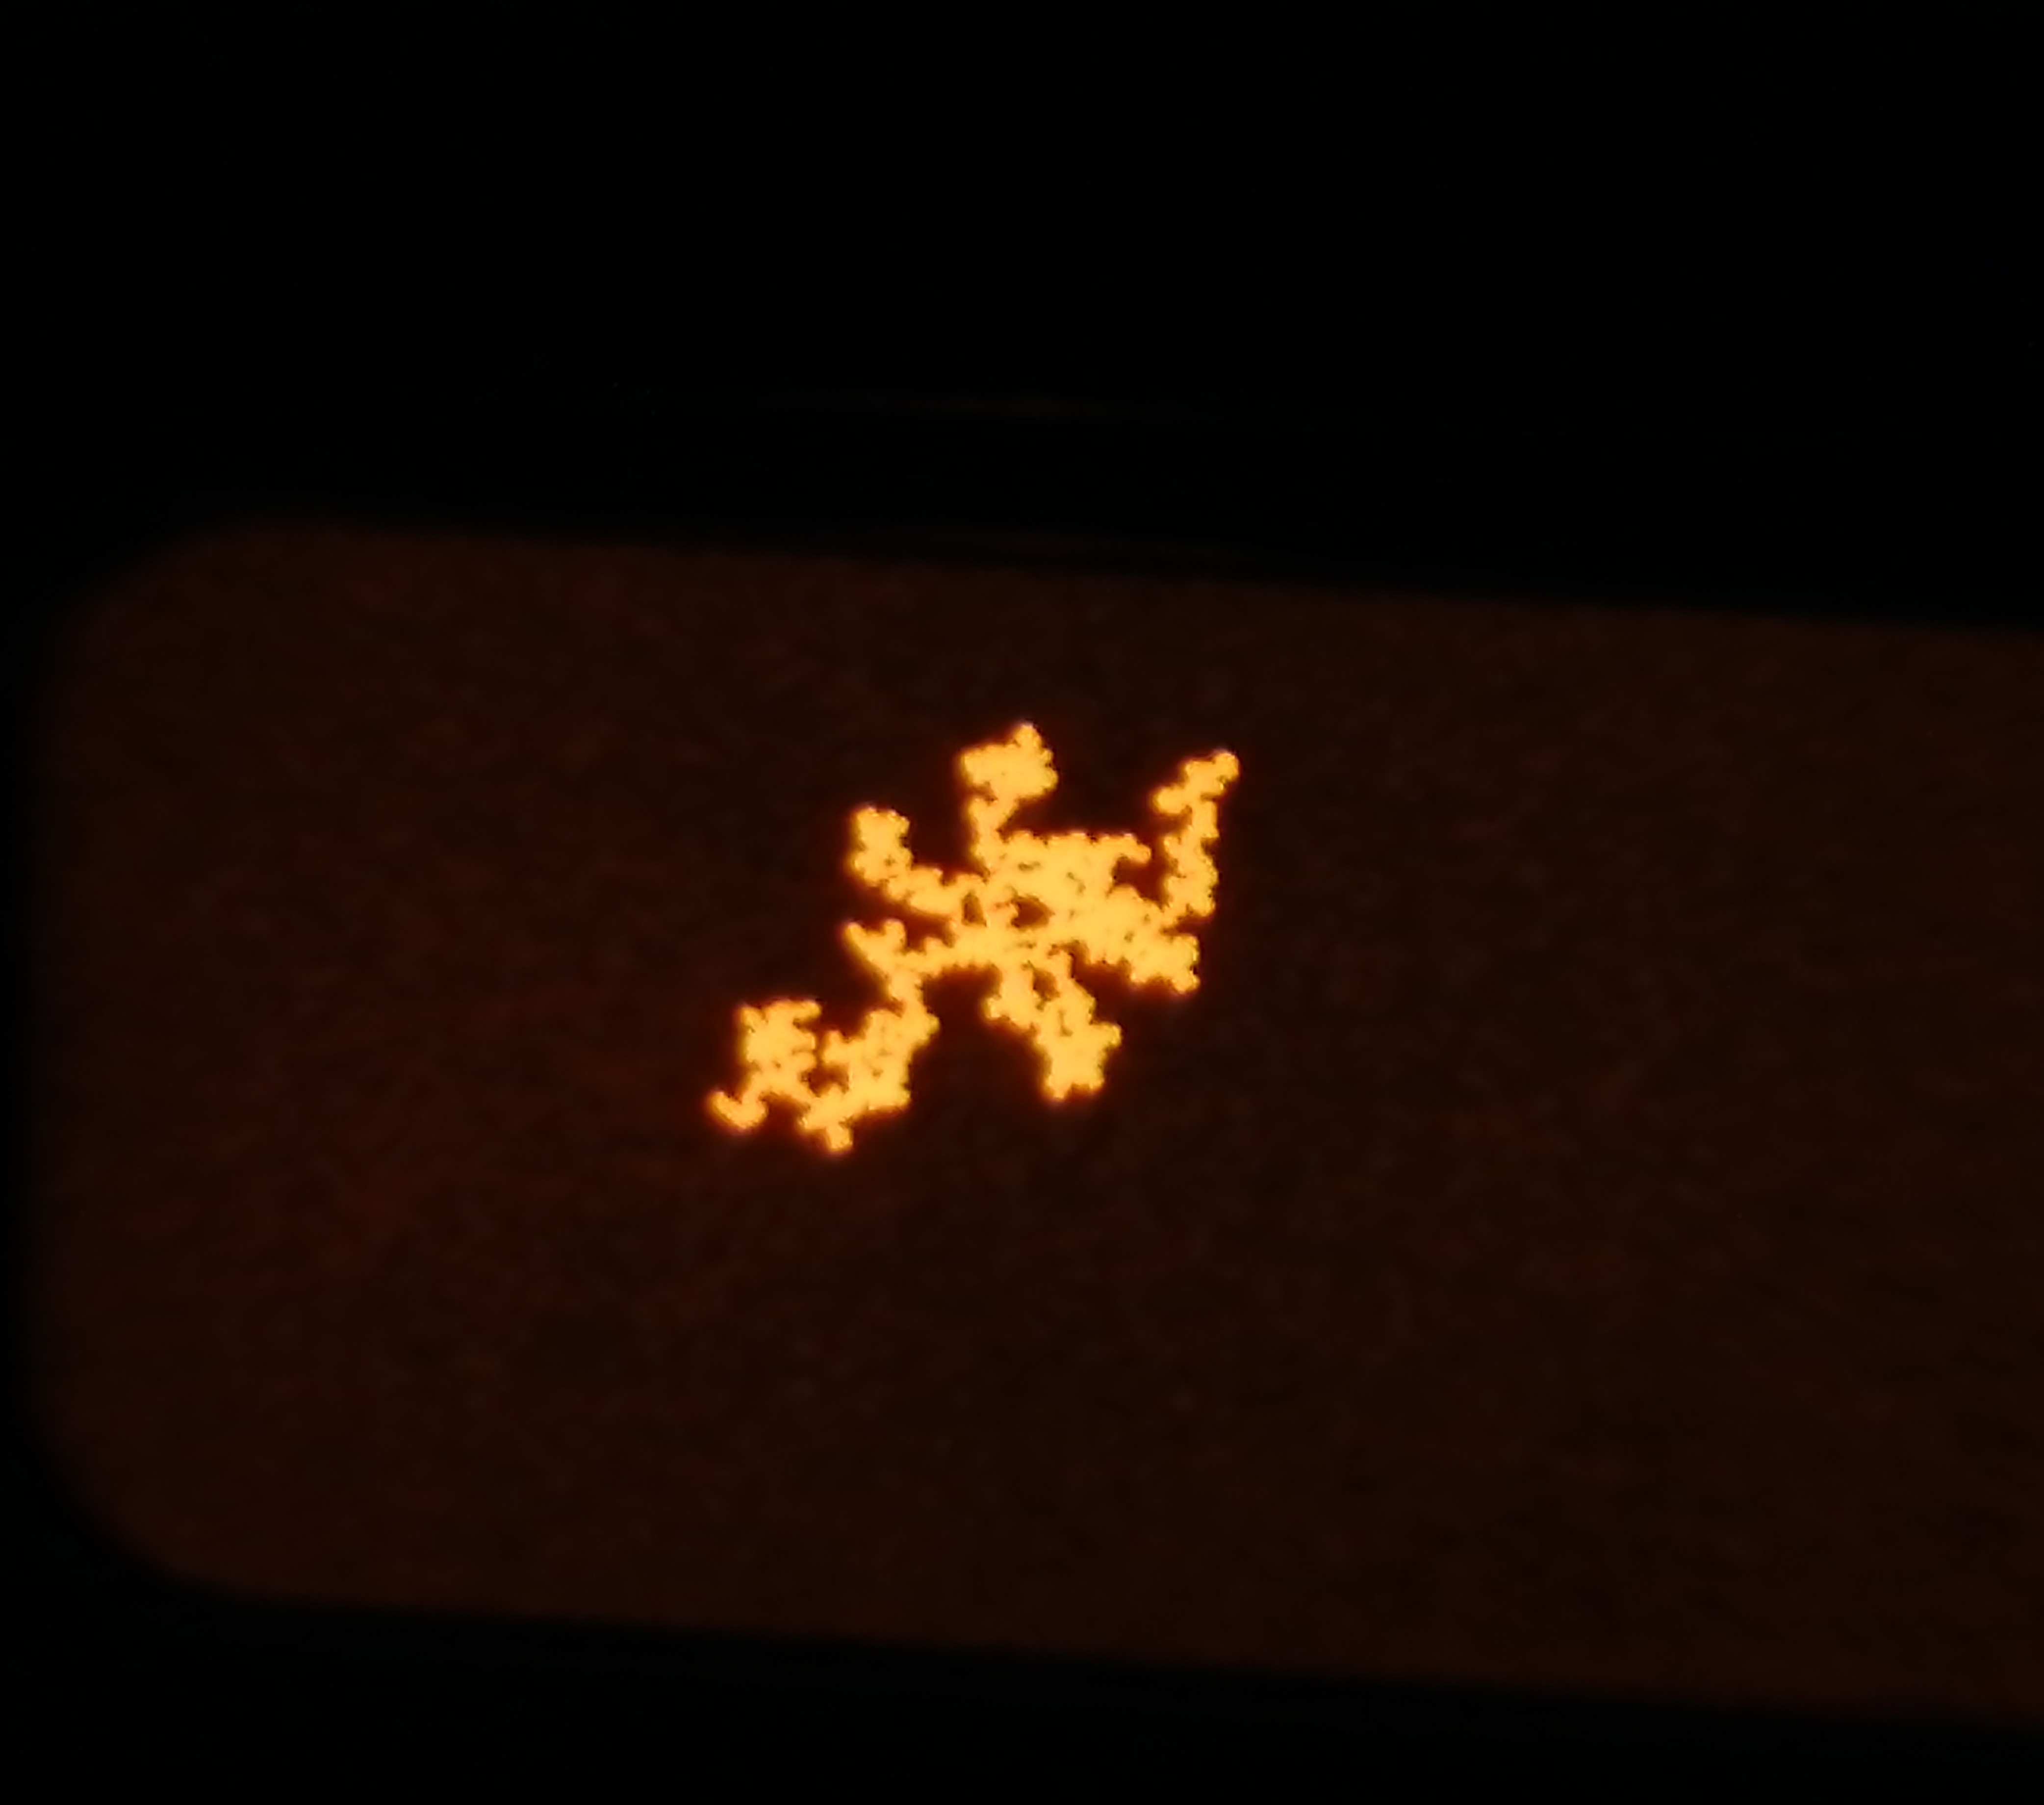
\includegraphics[scale=0.04]{display.jpg} 
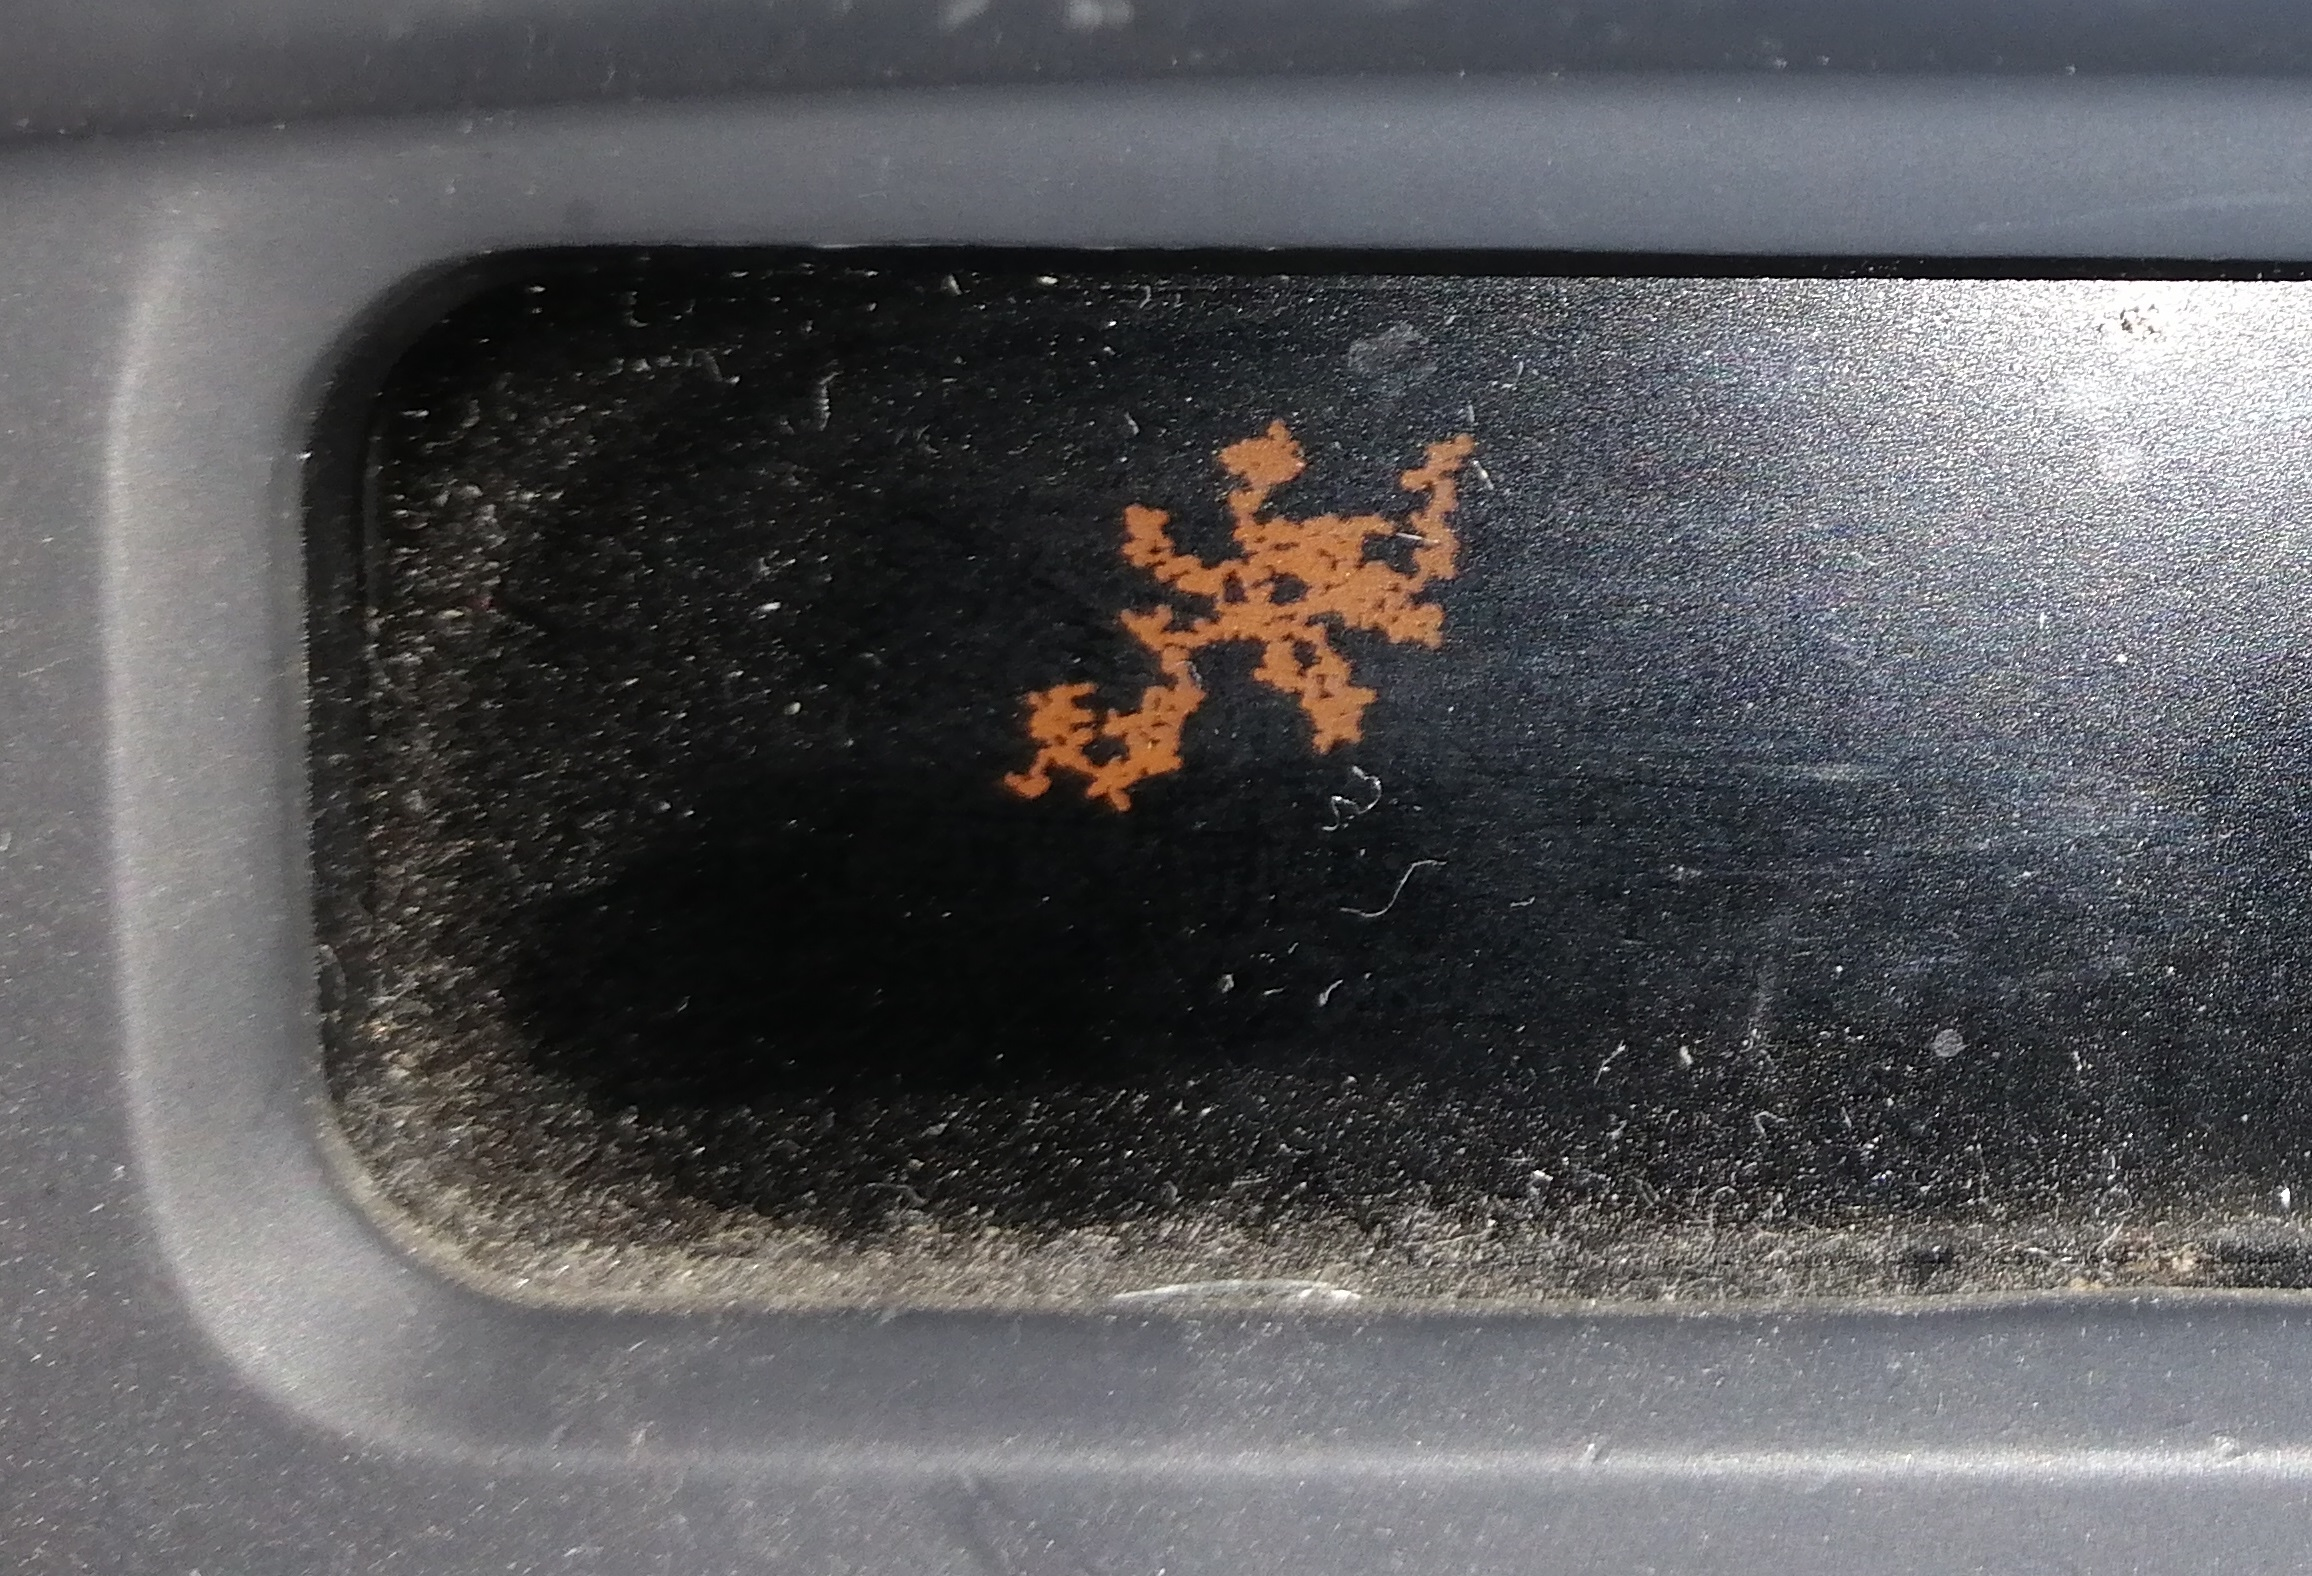
\includegraphics[scale=0.091]{display2.jpg}





\newpage


\section{Preliminaries} \label{prelim}

\subsection{Symbols}
Here we list all Symbols which will be used in this paper. Let $d\in \N$ and $q\in \{0,\dots,d\}$. 
\begin{flalign*}
	&\N = \{1,2,3,\dots\},\quad \text{the set of natural numbers (without 0)}\\
	&\N_0 = \N\cup\{0\}\\
	&\mathcal{B}^d,\quad \text{$d$-dimensional Borel-$\sigma$-algebra of $\R^d$} \\
	&\K^d,\quad \text{the set of convex and compact sets in }\R^d\\
	&B_d(r,x) = \{y\in \R^d\ |\ |x-y| \leq r\},\quad  \text{the $d$-dimensional closed ball of radius $r$ around $x$}\\
	&B_r := B_2(r,0) \\
	&S_{d-1}(r,x) = \partial B_d(r,x),\quad  \text{the $(d-1)$-dimensional surface of the $d$-dimensional ball}\\
	&A(d,q),\quad \text{the set of q-dimensional affine subspaces of }\R^d \\
	&\mathcal{A}(d,q),\quad  \text{the $\sigma$-algebra of } A(d,q), \text{ as constructed later in the paper} \\
	&\G := A(2,1),\quad  \text{the set of lines in the real plane}\\
	&SO_d := \{\nu \in \R^{d\times d}\ |\ \nu \nu^\top = I_d \text{ and } \det \nu = 1\},\quad \text{identify }SO_2 = \{\nu_\beta := e^{i\beta} \in \C\ |\ \beta\in [0,2\pi)\} \\
	&G_d := \{\varphi: \R^d \to \R^d, x\mapsto \nu x+b\ |\ \nu \in SO_d,b\in \R^d\},\quad  \text{the set of euclidean motions} \\
\end{flalign*}

\newpage
\subsection{Basic structures}

We prepare this script with the following preliminaries. Let $d\in \N$. \\

\noindent $\boldsymbol{\mathit{Graphs}}.\quad$ We will be interested in the graph $(\mathbb{Z}^d, E)$ with its canonical graph structure, which is two vertices (or points) $x=(x_1,\dots,x_d),y=(y_1,\dots,y_d)\in \mathbb{Z}^d$ form an edge (e.q. $\{x,y\}\in E$) if and only if there exists exactly one $i\in \{1,\dots, d\}$ such that $|x_i - y_i| = 1$ and $x_j = y_j$ for all $j\neq i$. For a point $x\in \mathbb{Z}^d$ its set of $\mathit{neighbours}$ is defined as 
\begin{align*}
	N(x) := \{y\in \mathbb{Z}^d\ |\ (x,y)\in E\}.
\end{align*}
For a set $A\subset \mathbb{Z}^d$ the $\mathit{outer\ boundary}\ \partial A$ of $A$ is defined as 
\begin{align*}
	\partial A := \{y\in \mathbb{Z}^d\setminus A\ |\ \exists x\in A:\ (x,y)\in E\}
\end{align*}
Instead of $(\mathbb{Z}^d, E)$ we will write $\mathbb{Z}^d$ from now on. 
\\

\noindent $\boldsymbol{\mathit{Probability\ Space}}.\quad$ Let $(\Omega,\mathcal{F}, \mathbb{P})$ be a probability space. For our space of interest $\mathbb{Z}^d$ we will always use the discrete $\sigma$-algebra which is the power set of $\mathbb{Z}^d$. If for $A\in \mathcal{F}$ we have $\mathbb{P}(A)=1$ we will say that "$A$ holds $\mathbb{P}$-$a.s.$", or short "$A$ holds $a.s.$" (almost sure).
\\

\noindent $\boldsymbol{\mathit{Random\ Walk}}.\quad$ A family $(S_n)_{n\in \mathbb{N}}$ of measurable functions $S_n: \Omega \to \mathbb{Z}^d$ is called a $\mathit{Random\ Walk\ on}\ \mathbb{Z}^d$ $\mathit{(starting\ at}\ x\in \mathbb{Z}^d)$ if and only if $S_0=x$, $a.s.$ and 

\begin{align*}
	\mathbb{P}(S_n = y\ |\ S_{n-1} = z) = \frac{1}{|N(z)|} = \frac{1}{2d},\quad \text{ for all }  y\in N(z) \text{ and } z\in \Z^d.
\end{align*}

\noindent Note that $|N(z)| = 2d$ for all $z\in \mathbb{Z}^d$ since every point has two neighbours in every dimension. We can therefore follow easily that $\mathbb{P}(S_n = y\ |\ S_{n-1} = z) = 0$ for all $y\notin N(z)$ and $z\in \Z^d$. So a Random Walk can be understood as a particle starting from some point $x$ and moving randomly on the grid choosing its next step uniformly from its neighbours. Further define 

\begin{align*}
	\mathbb{P}_x(S_n\in A) := \mathbb{P}(S_n\in A|S_0=x)
\end{align*}

\noindent for any subset $A\subset \Z^d$. We define the $hitting\ times$ of A by

\begin{align*}
	T_A := \min \{n\geq 0\ |\ S_n\in A\}\text{ and } T^+_A := \min \{n\geq 1\ |\ S_n\in A\}, 
\end{align*}

\noindent $T_x:= T_{\{x\}}$ and $T^+_x:= T^+_{\{x\}}$ for one element sets and $x\in \Z^d$. The $heat\ kernel$ of the random walk $S_n$ is defined to be 

\begin{align*}
	p_n(x,y):=\mathbb{P}_x(S_n=y)
\end{align*}

\noindent and the $\mathit{Green\ function}$ as 

\begin{align*}
	G(x,y) := \sum_{n\geq 0} p_n(x,y).
\end{align*}

$G$ is well-defined and finite since $\Z^2$ is transient. Similarily for a subset $A\subset G$ the $killed$ or $\mathit{stopped\ Green\ function}$ is defined as

\begin{align*}
	G_A(x,y) := \sum_{n\geq 0} \mathbb{P}_x(S_n=y, T_A > n).
\end{align*} 



\newpage
\section{Incremental Aggregate}
In this paper we will look at stochastic processes on the set of finite subsets of $\mathbb{Z}^d$, where we start with a one point set at $\{0\}$ and incrementally add a point on the outer boundary of the current cluster according to some distribution. What we get is a randomly, point by point growing connected cluster which we will call $\mathit{Incremental\ Aggregate}$. Define 
\begin{align}
	\mathcal{P}_f := \{A\subset \mathbb{Z}^d\ |\ \text{A is finite}\}, 
\end{align}
the set of finite subsets of $\mathbb{Z}^d$. Furthermore we will be interested in distributions on those sets, so for $A\in \mathcal{P}_f$ we define 
\begin{align}
	\mathcal{D}_A:= \{\mu: \mathbb{Z}^d\to [0,1]\ |\ \mu(y) = 0 \text{ for all } y\notin A\ \text{and}\ \sum_{y\in A} \mu(y) = 1 \}, 
\end{align}
the set of distributions on $A$. Now we define $\mathit{Incremental\ Aggregate}$ as follows.  

\begin{definition}
	Let $\mu=(\mu_A)_{A\in \mathcal{P}_f}$ be a family of distributions with $\mu_A\in \mathcal{D}_A$ for all $A\in \mathcal{P}_f$. $\mathit{Incremental\ Aggregate\ (with\ distribution\ \mu)}$ is a stochastic process $(\mathcal{E}_n)_{n\in{\mathbb{N}_0}}$ which evolves as follows. The process starts with one point $\mathcal{E}_0 = \{0\}$ at the origin of $\mathbb{Z}^d$. Knowing the process $\mathcal{E}_n$ at time $n$, let $y_n$ be a random point in $\partial \mathcal{E}_n\in \mathcal{P}_f$ with distribution
	\begin{align}
		\mathbb{P}(y_n = y\ |\ \mathcal{E}_n) := \mu_{\partial \mathcal{E}_n}(y),\quad y\in \mathbb{Z}^d.
	\end{align}
	We then define $\mathcal{E}_{n+1} := \mathcal{E}_n \cup \{y_n\}$.
\end{definition} 

For all incremental aggregates in this paper we will have $d=2$. From now on we will identify $\R^2$ with $\C$ as $\R$-vectorspaces. 




\newpage

\newpage
\section{External DLA}

External DLA is a model of an Incremental Aggregate as defined above using a very natural family of distributions, called the $\mathit{harmonic\ measures}$. 

\begin{definition} $\mathit{(Harmonic\ Measure)}$ Let $A\in\mathcal{P}_f$. Remembering the definitions in \eqref{prelim}, especially the heat kernel $p_n(x,y)=\mathbb{P}_x(S_n=y)$ of a random walk, for $x\in \Z^2$ the $\mathit{harmonic\ measure}$ (from $x$) of $A$ is
	\begin{align*}
	h_A(x,y) := \1\{y\in A\}p_{T_A}(x,y) = \1\{y\in A\}\PP_x(S_{T_A} = y),\quad \text{ for } y\in \Z^2.  
	\end{align*}
	We now define the $\mathit{harmonic\ measure}$ (from infinity) of $A$ as the family $h=(h_A)_{A\in \mathcal{P}_f}$ with
	\begin{flalign*}
		h_A(y) := \lim_{|x|\to\infty} h_A(x,y),\quad y\in \Z^2. 
	\end{flalign*}
	This is well-defined because ... CONTINUE
\end{definition}

\begin{definition} $\mathit{(External\ Diffusion\ Limited\ Aggregate)}$ $\mathit{External\ Diffusion\ Limited\ Aggregate}$, short $\mathit{External\ DLA}$, is a incremental aggregate with the harmonic measure $h$ as distribution. 
\end{definition}



\newpage
\section{Integral Geometry}

In the next section we want to define an approximation for External DLA. This approximation will be an incremental aggregate for which distribution definition we need some concepts and results from Integral Geometry which we will discuss and develop in this section. In the process we want to define we will want to choose a random line out of all lines which intersect with the current cluster of the aggregate. This random choosing is not obvious since most of the time the cluster will be strongly non symmetric and it is even less obvious how to actually get a realisation of a random line when simulating with Python. In our case we are looking for a parametrisation of lines in the plane and a reasonable way of choosing parameters randomly. \\

We will introduce a possible solution for this problem first through the abstract and general concepts of integral geometry and later through a simple parametrisation for the case of lines in the plane which goes hand in hand with the general result.
 
\subsection{General results}

In the general context we are in $\R^d$ for $d\in \N$ and consider $q$-dimensional affine subspaces where $q\in \{0,\dots,d\}$, short $q$-flats in $\R^d$. The set of $q$-flats in $\R^d$ is denoted by $A(d,q)$. Later we will be interested in choosing random lines in the real plane (i.e. $1$-flats in $\R^2$). In order to get a probability measure on some set of $q$-flats, we first need a measure and a $\sigma$-algebra on $A(d,q)$ in total. 

\begin{definition}
	For $B\in \mathcal{B}^d$ define 
	\begin{flalign*}
		[B]_{d,q} := \{F\in A(d,q)\ |\ F\cap B \neq\emptyset\}.
	\end{flalign*}
	If the context is clear, we will only write $[B]$ instead of $[B]_{d,q}$. 
\end{definition}

\begin{definition}
	The $\sigma$-algebra $\mathcal{A}(d,q)$ on $A(d,q)$ is defined by
	\begin{flalign*}
		\mathcal{A}(d,q) := \sigma(\{ [K]\ |\ K\in \K^d\}).
	\end{flalign*} 
\end{definition}

\begin{theorem} \label{uniqmeas}
	On $A(d,q)$ there exists a unique $G_d$-invariant Radon measure $\mu_q$ such that
	\begin{flalign}
		\mu_q(A_{B_d(1,0)}) = \kappa_{d-q}, 
	\end{flalign}
	where $\kappa_n := \lambda_n(B_n(1,0))$ is the $n$-dimensional Lebesque meausure of the $n$-dimensional unit ball for $n\in \N$, and $\kappa_0:=1$.
\end{theorem}
\begin{proof}
	\cite{stoch1} Theorem 4.26 \\ \\ MAKE PROOF CLEARER
\end{proof}

\subsection{Construction in the plane: Isotropic lines}

For our special case we choose $d=2$ and $q=1$, thus lines in the plane. We denote this set of lines by $\G$. The following construction in this chapter is completely motivated by \cite{sackmann} 2.1.1. Firstly we propose a parametrisation of lines which works as follows. Every line can be uniquely determined by an angle $\alpha\in [0,\pi)$ and a real number $p\in \R$. Let $\langle\cdot,\cdot\rangle$ be the standard scalar product on $\R^2$, respectively used for values in $\C$ as we identify $\R^2$ with $\C$ as $\R$-vectorspaces. Let $e_\alpha := e^{\alpha i} = \cos(\alpha) + \sin(\alpha)i$ and $s_\alpha : = -\sin(\alpha) + \cos(\alpha)i$ be the unit vectors $1$ and $i$ rotated by $\alpha$ counterclockwise. Lets consider the representation $x = \langle x,e_\alpha\rangle e_\alpha + \langle x,s_\alpha\rangle s_\alpha$ for $x\in \C$. Since $e_\alpha$ and $s_\alpha$ form a base of $\C$ as a $\R$-vectorspace, the parameters $\langle x,e_\alpha\rangle$ and $\langle x, s_\alpha\rangle$ are unique for each $x$. It thus is easy to realize that $g_{\alpha,p} := \{x\in \C\ |\ \langle x,e_\alpha\rangle  = p\}$ defines a line (compare with $\autoref{lineparam}$) and that every line has a unique pair of $\alpha$ and $p$ for such a representation. In words, $g_{\alpha,p}$ contains all points which have length $p$ in direction of $e_\alpha$. With $\Phi := [0,\pi) \times \R$ this naturally defines a bijection
\begin{flalign*}
	\chi: \Phi \to \G, \quad (\alpha,p) \mapsto g_{\alpha,p}. 
\end{flalign*}
\\
\begin{figure}
	\centering
	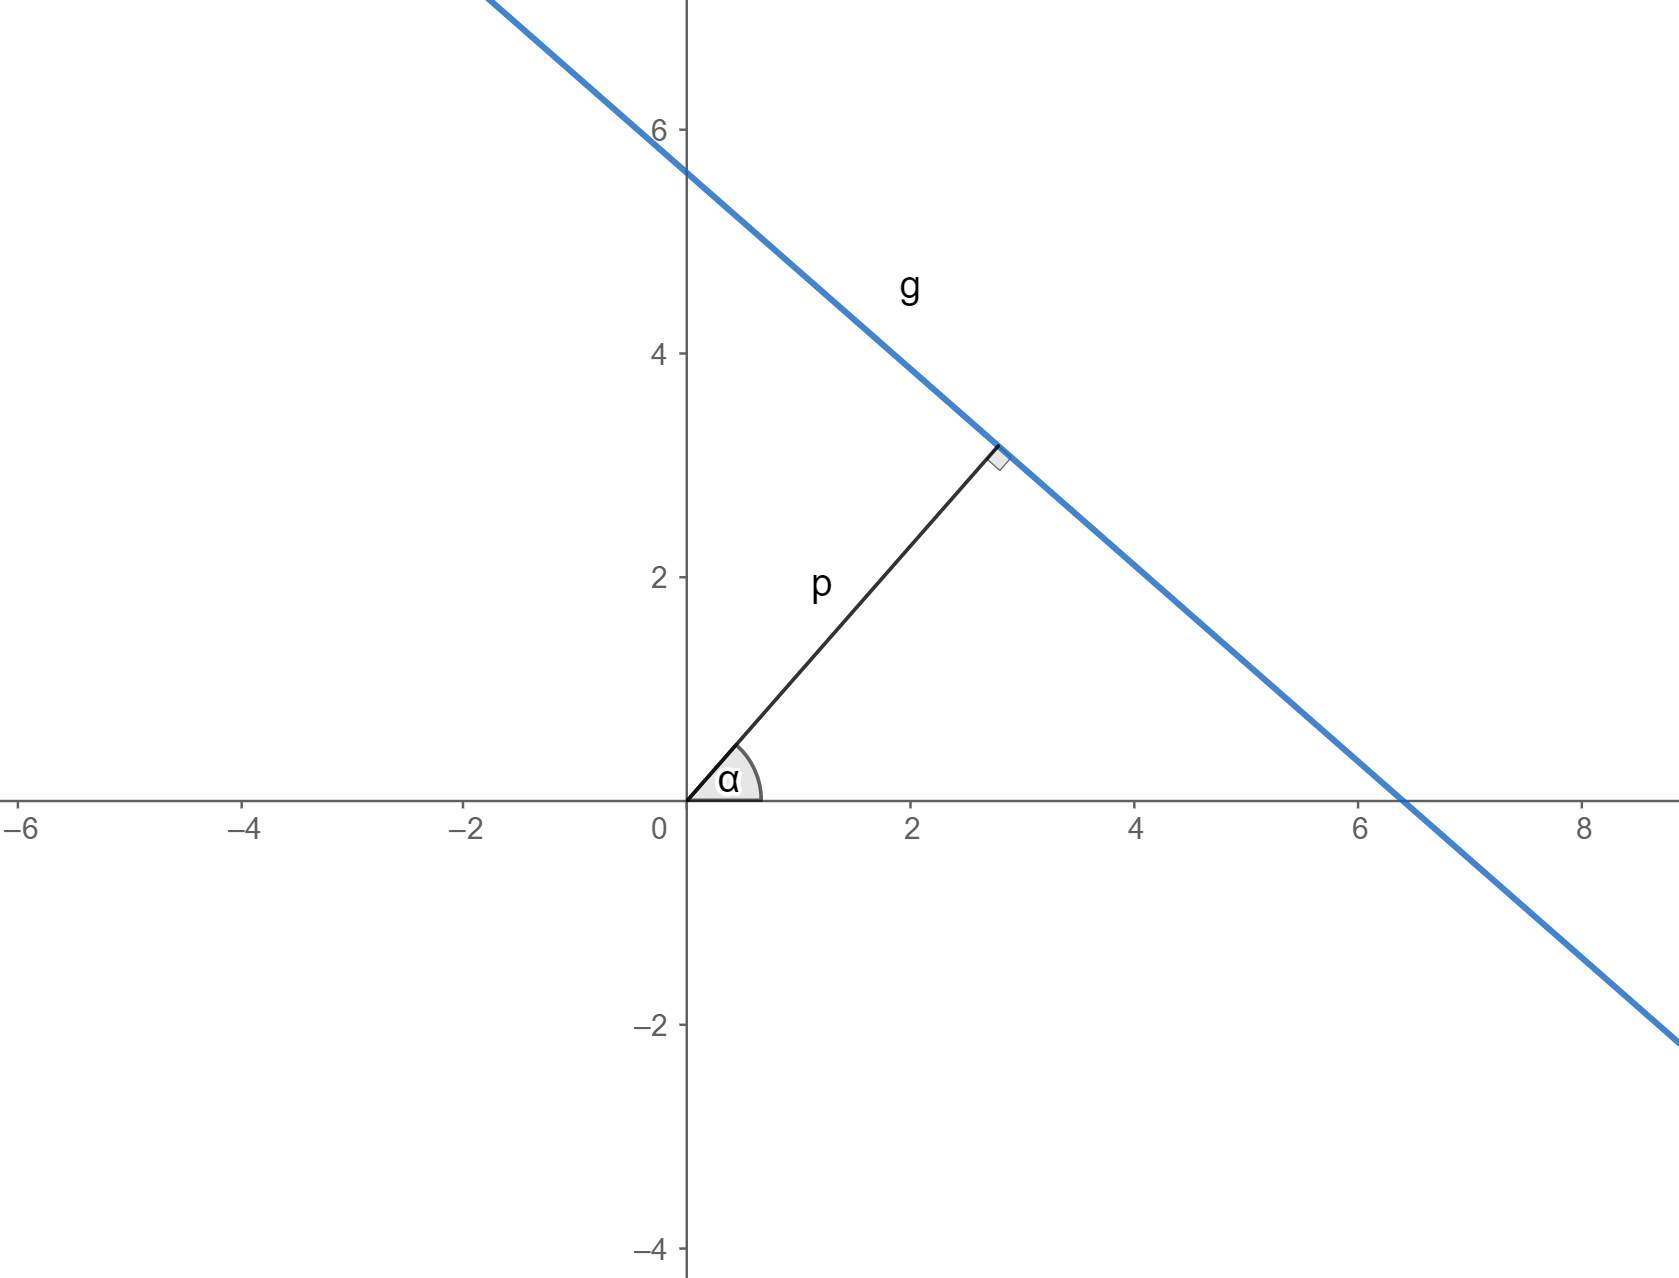
\includegraphics[height=10cm]{line-param.png}
	\caption{Line parameters $\alpha$ and $p$} \label{lineparam}
\end{figure}
\\


We take the subspace Borel-$\sigma$-algebra $\mathcal{B}_\Phi:= \mathcal{B}^2 \cap \Phi$ on $\Phi$ and define the $\sigma$-algebra $\GG$ on $\G$ by $\GG := \chi(\mathcal{B}_\Phi)$. This works well since $\chi$ is a bijection. The next lemma shows that this way of defining a $\sigma$-algebra on $\G$ makes sense as it is indeed equivalent to the general context as defined above. 

\begin{lemma}
	We have $\mathcal{A}(2,1) = \GG$. 
\end{lemma}
\begin{proof}
	To proof this it is helpful to consider generators of these $\sigma$-algebras. Define the set of closed rectangles in $\Phi$ as $\mathcal{R} := \{[\alpha,\beta] \times (c,d]\subset \Phi\ |\ 0\leq \alpha<\beta<\pi,c<d\}$. Then by measure theory we know that $\mathcal{B}_\Phi = \sigma (\mathcal{R})$ and since $\chi$ is a bijection, we have $\chi(\sigma (\mathcal{R})) = \sigma (\chi(\mathcal{R}))$ and finally $\GG = \sigma(\chi(\mathcal{R}))$. For $\tilde A := \{[K]\ |\ K\in \K^2\}$ we have by definition $\mathcal{A}(2,1) = \sigma(\tilde A)$. \\
	%
	\\ \indent $\subset$: Let $K\in\K^2$. We will show that $\chi^{-1}([K])$ is a closed set in $\Phi$. If that is the case we have $\chi^{-1}([K])\in\mathcal{B}_\Phi$, therefore $[K] \in\chi(\mathcal{B}_\Phi) = \GG$ and finally $\mathcal{A}(2,1) = \sigma(\tilde A)\subset\GG$. To show that $\chi^{-1}([K])$ is a closed let $(\alpha_0,p_0)\in \Phi\setminus \chi^{-1}([K])$. Then $\chi(\alpha_0,p_0) \notin [K]$ and therefore $\chi(\alpha_0,p_0) \cap K= \emptyset$. Since $K$ is closed we can find small values $\tilde\alpha,\tilde p > 0$ such that $\chi(\alpha,p) \cap K = \emptyset$ for all $(\alpha,p)\in [\alpha_0, \alpha_0 + \tilde\alpha] \times [p_0, p_0 + \tilde p] =: R$. Hence we have $ R\subset \Phi \setminus \chi^{-1}([K])$, so $\Phi \setminus \chi^{-1}([K])$ is open. Hence $\chi^{-1}([K])$ is closed. \\
	%
	\\ \indent $\supset$: For this inclusion we will show that $\chi(R)\in\mathcal{A}(2,1)$ for all $R\in\mathcal{R}$. Recall that $\sigma$-algebras are closed under countable unions per definition and further closed under substraction ($A\setminus B\in \mathcal{A}(2,1)$ for all $A,B\in \mathcal{A}(2,1)$). Let $b>0$. For a general rectangle $R=[\alpha,\beta] \times (a,b]$ with $a\neq 0$ we can write $R= [\alpha,\beta]\times(0,b]\cup [\alpha,\beta]\times(a,0]$ and therefore $\chi(R) = \chi([\alpha,\beta]\times(0,b])\cup\chi([\alpha,\beta]\times(a,0])$ in case of $a<0$, and $R = ([\alpha,\beta]\times(0,b])\setminus([\alpha,\beta]\times(0,a])$ and therefore $\chi(R) = \chi([\alpha,\beta]\times(0,b])\setminus\chi([\alpha,\beta]\times(0,a])$ in case of $a>0$. Analog results we get for $b<0$. So in total we only have to show $\chi(R) \in\mathcal{A}(2,1)$ for rectangles of the forms $[\alpha,\beta]\times(0,b]$ and $[\alpha,\beta]\times(b,0]$, $b\neq 0$. So without loss of generality let $b>0$ and $R = [\alpha,\beta]\times(0,b]$. Define 
	\begin{flalign*}
		S:= \{pe_\gamma \in \C\ |\ (\gamma,p)\in R\}
	\end{flalign*}
	Furthermore for $n\in \N$ define 
	\begin{flalign*}
		A_n := \{tns_\beta\ |\ t\in [0,1]\} \text{ and } B_n := \{-tns_\alpha\ |\ t\in [0,1]\},
	\end{flalign*}
	the segments from $0$ to $ns_\beta$ and $0$ to $-ns_\alpha$ ($\autoref{circleS}$). We will show now that 
	\begin{flalign*}
		\chi(R) = [S] \setminus (\bigcup_{n\in\N} [A_n] \cup \bigcup_{n\in\N} [B_n]) =: \tilde S. 
	\end{flalign*}
	\\
	Let $(\gamma,p)\in R$. Then $pe_\gamma\in \chi(\gamma,p)\cap S$ and therefore $\chi(\gamma,p)\in [S]$. Assume that there exits a $n\in\N$ such that $\chi(\gamma,p)\cap A_n \neq \emptyset$. Then $\beta + \frac{\pi}{2} - \gamma < \frac{\pi}{2}$, hence $\beta < \gamma$, a contradiction. Similairly argument for any $B_n$, so we finally have $\chi(\gamma,p) \notin [A_n]$ and $\chi(\gamma,p) \notin [B_n]$ for any $n\in \N$. Hence $\chi(R)\subset \tilde S$. \\
	\\
	Now let $(\gamma,p)\in\Phi$ such that $\chi(\gamma,p)\in \tilde S$. Assume that $\gamma\notin[\alpha,\beta]$ then with a similair arguemnt as in the first inclusion it is easy to see that there must be $n\in\N$ such that $\chi(\gamma,p)\cap A_n\neq \emptyset$ or $\chi(\gamma,p)\cap B_n\neq \emptyset$, a contradiction. Therefore $\gamma\in[\alpha,\beta]$. Now assume $p\notin (0,b]$. If $p>b$ then $\chi(\gamma,b)\cap B_b = \emptyset$ and since $S\subset B_b$ it is $\chi(\gamma,p)\notin [S]$, a contradiction. If $p<0$ then since the angle between the segments $A_n$ and $B_n$ for some $n\in \N$ opposite of $S$ is strictly smaller than $\pi$ and therefore $\chi(\gamma,p)$ must intersect with $A_n$ or $B_n$ for some $n\in\N$, again a contradiction. Thus we have $p\in(0,b]$. Therefore we have $(\gamma,p)\in R$ and finally $\tilde S\subset \chi(R)$. 
	\\
	If is left to show that $\tilde S\in \mathcal{A}(2,1)$. All the segments $A_n$ and $B_n$ are compact and convex for all $n\in\N$, and also 
	

	CONTINUE
\end{proof}

\begin{figure}
	\centering
	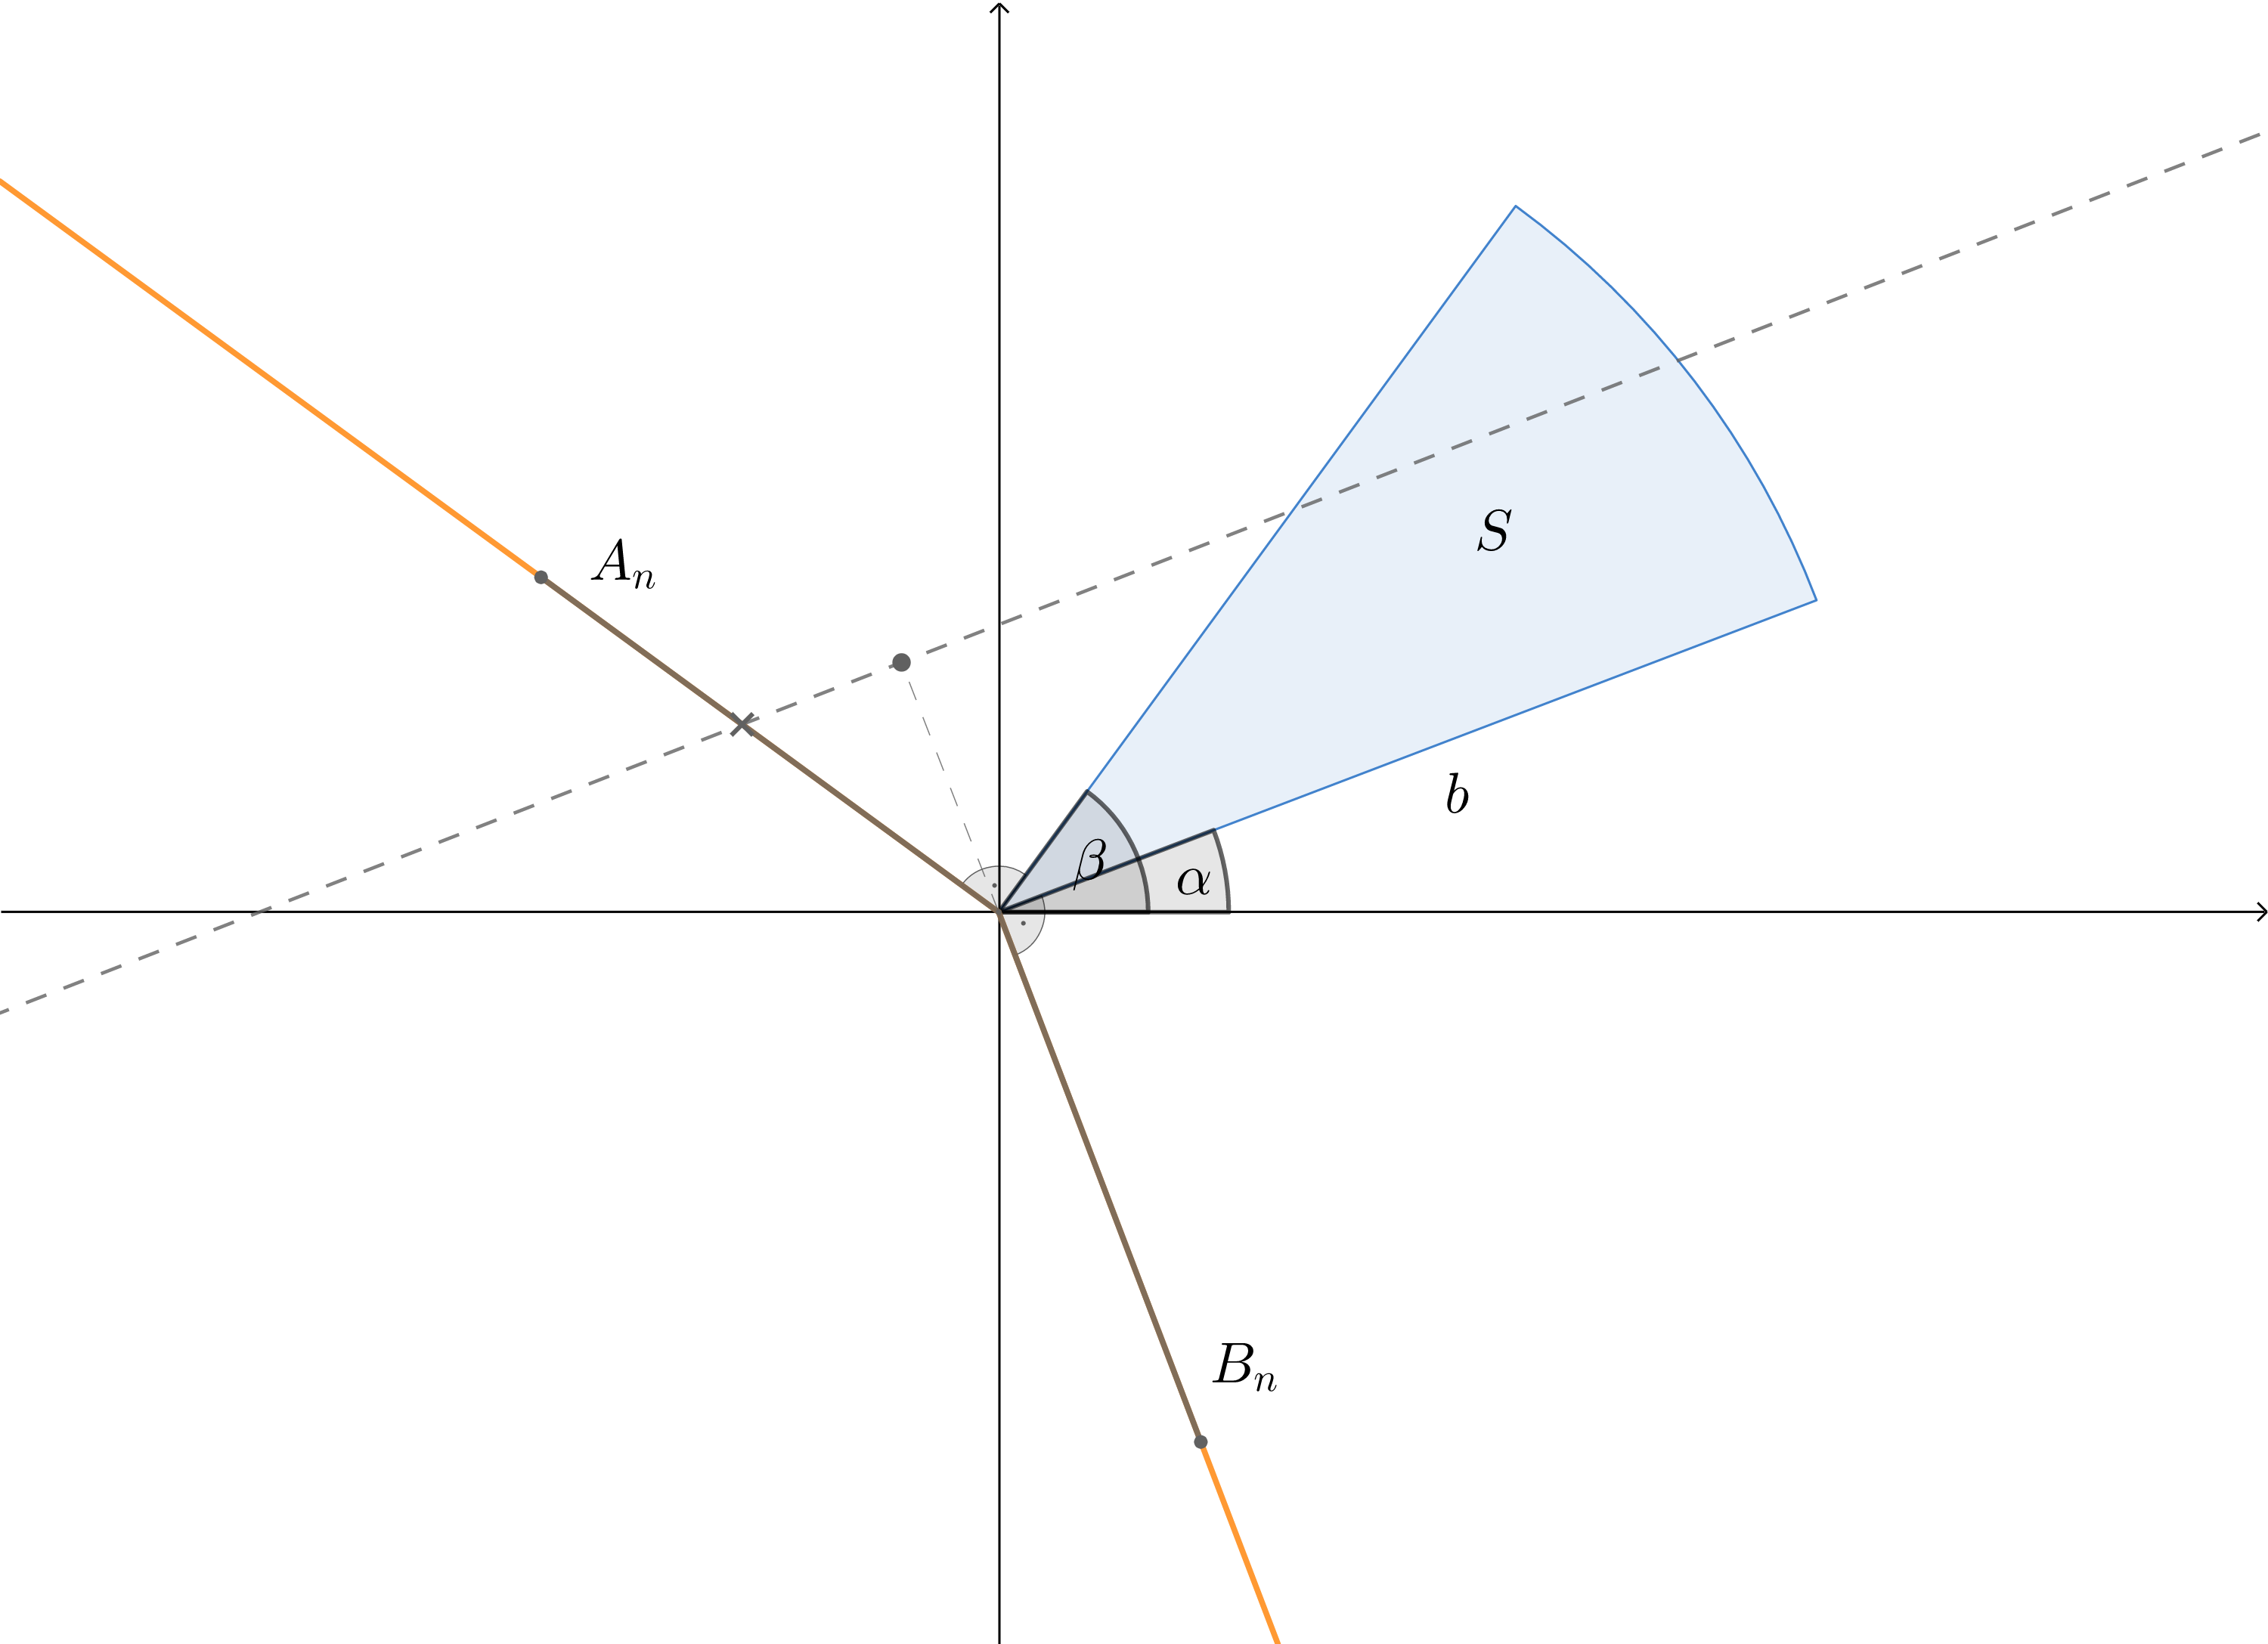
\includegraphics[height=10cm]{circle-part-S.png}
	\caption{$S$ and the sets $A_n$ and $B_n$} \label{circleS}
\end{figure}


\begin{definition}
	A $\mathcal{F}$-$\GG$-measurable function $g:\Omega \to \G$ is called a $\mathit{random\ line}$.  
\end{definition}

\begin{definition}
	We define the measure $\mu := {\lambda_2}_{|\Phi} \circ \chi^{-1}$ on $(\G,\GG)$ where ${\lambda_2}_{|\Phi}$ is the $2$-dimensional Lebesgue measure restricted to $\Phi$. We say a measure $\nu$ on $(\G,\GG)$ is locally finite if for any $K\in \K^2$ we have $\nu([K])<\infty$. 
\end{definition}

\begin{lemma}
	$\mu$ is locally finite and $G_2$-invariant. 
\end{lemma}
\begin{proof}
	Let $K\in \K^2$ and since $K$ is compact choose $r> 0$ such that $K\subset B_r$. Then we have $[K]\subset A_{B_r}$ and
	\begin{flalign*}
		\mu([K]) \leq \mu(A_{B_r}) = {\lambda_2}_{|\Phi} (\chi^{-1}(A_{B_r})) = {\lambda_2}_{|\Phi}([0,\pi)\times [-r,r]) = 2\pi r < \infty, 
	\end{flalign*}
	hence $\mu$ is locally finite. To show that $\mu$ is $G_2$-invariant, that means euclidean motion invariant, we must show it is translation and rotation invariant. First we clarify what exactly translation and rotation mean for lines. We denote $x\ modulo\ r$ as $(x)_r$. For $b\in\C$ and $\beta\in[0,2\pi)$ we define 
	\begin{flalign} \label{motion}
		T_b:\ &\Phi \to \Phi,\quad (\alpha,p) \mapsto (\alpha,p+\langle e_\alpha, b\rangle)
	\end{flalign}
	and
	\begin{flalign} \label{motion2}
	D_{\beta}:\ &\Phi \to \Phi,\quad (\alpha,p) \mapsto ((\alpha + \beta)_{\pi}, \delta((\alpha + \beta)_{2\pi})p), 
	\end{flalign}
	where 
	\begin{flalign*}
		\delta: [0,2\pi) \to \{-1,1\}, \quad \gamma \to \begin{cases}
			1,\ \gamma\in [0,\pi) \\
			-1,\ \gamma\in [\pi,2\pi)
		\end{cases}.
	\end{flalign*}
	It is easy to see that both functions all well-defined. $T_b$ defines a translation by $b$ and $D_\beta$ a rotation by $\beta$. Lets proof that first. Let $(\alpha,p)\in \Phi$, then 
	\begin{flalign*}
		x\in \chi(\alpha,p)+b &\Leftrightarrow x-b\in \chi(\alpha,p) \\ 
		&\Leftrightarrow \langle e_\alpha, x-b\rangle = p \\ 
		&\Leftrightarrow \langle e_\alpha, x\rangle = p + \langle e_\alpha, b\rangle \\
		&\Leftrightarrow x\in \chi(\alpha, p + \langle e_\alpha, b\rangle) \\
		&\Leftrightarrow x\in \chi(T_b(\alpha, p))
	\end{flalign*}
	and therefore $\chi(\alpha,p) + b = \chi(T_b(\alpha, p))$. Hence $T_b(\alpha,p)$ are indeed the parameters for the by $b$ translated line. For the rotation lets devide it into two cases. First let $(\alpha+\beta)_{2\pi} \in [0,\pi)$, then $\delta((\alpha+\beta)_{2\pi}) = 1$ and $(\alpha+\beta)_\pi = \alpha+\beta$ and therefore 
	\begin{flalign*}
		D_\beta(\alpha,p) = (\alpha+\beta,p).
	\end{flalign*} 
	In the second case with $(\alpha+\beta)_{2\pi} \in [\pi,2\pi)$ we have $\delta((\alpha+\beta)_{2\pi}) = -1$ and $(\alpha+\beta)_\pi = \alpha+\beta - \pi$ and therefore
	\begin{flalign*}
		D_\beta(\alpha,p) = (\alpha + \beta - \pi, -p).
	\end{flalign*}
	In the second case we have to carefully understand the parametrisation of $\G$, but finally we can see that $D_\beta(\alpha,p)$ are indeed the parameters of the by $\beta$ rotated line. \\
	\\We will further show now, that $\mu$ is invariant in respect to both these functions. Let $A\in \GG$, $b\in \C$ and $\nu_\beta\in SO_2$ for some $\beta\in[0,2\pi)$. We will understand $A+b = \{g+b\in \G\ |\ g\in A\}$ and $\nu_\beta A = \{\nu_\beta g\in \G\ |\ g\in A\}$ pointwise, and $g+b = \{x+b\ |\ x\in g\}$ and $\nu_\beta g=\{\nu_\beta x\ |\ x\in g\}$ pointwise aswell. We furthermore define $A_p := \{\alpha\in[0,\pi)\ |\ (\alpha,p)\in \chi^{-1}(A)\}$ and $A_\alpha := \{p\in \R\ |\ (\alpha,p)\in \chi^{-1}(A)\}$ for $(\alpha,p)\in \Phi$. For a translation we get 
	\begin{flalign*}
		\mu(A+b) 
		&= \int_\GG \1_{A+b}(g) \mu(dg) \\
		&= \int_\GG \1_A(g-b) \mu(dg) \\
		&= \int_\GG \1_A(g-b) {\lambda_2}_{|\Phi}(\chi^{-1}(dg)) \\
		&= \int_{\chi^{-1}(\GG)} \1_{\chi^{-1}(A)}(\chi^{-1}(g-b)) {\lambda_2}_{|\Phi}(d(\chi^{-1}(g))) \\
		&\overset{(\ref{motion})}{=} \int_\Phi \1_{\chi^{-1}(A)}(\alpha,p-\langle e_\alpha, b\rangle) {\lambda_2}_{|\Phi}(d(\alpha,p)) \\ 
		&= \int_0^\pi \int_\R \1_{A_\alpha}(p-\langle e_\alpha, b\rangle) {\lambda_1}(dp){{\lambda_1}_{|[0,\pi)}}(d\alpha) \\ 
		&= \int_0^\pi \int_\R \1_{A_\alpha +\langle e_\alpha, b\rangle}(p) {\lambda_1}(dp){{\lambda_1}_{|[0,\pi)}}(d\alpha) \\ 
		&= \int_0^\pi \lambda_1(A_\alpha +\langle e_\alpha, b\rangle) {{\lambda_1}_{|[0,\pi)}}(d\alpha) \\ 
		&\overset{(+)}= \int_0^\pi \lambda_1(A_\alpha) {{\lambda_1}_{|[0,\pi)}}(d\alpha) \\ 
		&= \dots \\
		&= \mu(A),
	\end{flalign*}
	and for a rotation we get
	\begin{flalign*}
		\mu(\nu_\beta A) &= \int_\G \1_{\nu_\beta A}(g) \mu(dg) \\
		&= \int_\G \1_A(\nu_{-\beta} g) {\lambda_2}_{|\Phi}(\chi^{-1}(dg))\\
		&= \int_{\chi^{-1}(\G)} \1_{\chi^{-1}(A)}(\chi^{-1}(\nu_{-\beta} g)) {\lambda_2}_{|\Phi}(d(\chi^{-1}(g)))\\
		&\overset{(\ref{motion2})}= \int_\Phi \1_{\chi^{-1}(A)}((\alpha - \beta)_{\pi}, \delta((\alpha - \beta)_{2\pi})p) {\lambda_2}_{|\Phi}(\alpha,p) \\
		&= \int_\Phi \1_{\chi^{-1}(A)}((\alpha - \beta)_{\pi}, \delta((\alpha - \beta)_{2\pi})p) {\lambda_2}_{|\Phi}(\alpha,p) \\
		&= \int_{0}^{2\pi} \int_\R \1_{\chi^{-1}(A)}((\alpha - \beta)_{\pi}, \delta((\alpha - \beta)_{2\pi})p) {\lambda_1}(dp){{\lambda_1}_{|[0,\pi)}}(d\alpha) \\
		&= \int_{0}^{2\pi} \int_\R \1_{A_{(\alpha - \beta)_{\pi}}}(\delta((\alpha - \beta)_{2\pi})p) {\lambda_1}(dp){{\lambda_1}_{|[0,\pi)}}(d\alpha) \\
		&\overset{(+)}= \int_{0}^{2\pi} \int_\R \1_{A_{(\alpha - \beta)_{\pi}}}(p) {\lambda_1}(dp){{\lambda_1}_{|[0,\pi)}}(d\alpha) \\
		&= \int_\R \int_{0}^{2\pi} \1_{\chi^{-1}(A)}((\alpha - \beta)_{\pi}, p) {{\lambda_1}_{|[0,\pi)}}(d\alpha){\lambda_1}(dp) \\
		&= \int_\R \int_{0}^{2\pi} \1_{A_p}((\alpha - \beta)_{\pi}) {{\lambda_1}_{|[0,\pi)}}(d\alpha){\lambda_1}(dp) \\
		&\overset{(+)}= \int_\R \int_{0}^{2\pi} \1_{A_p}(\alpha) {{\lambda_1}_{|[0,\pi)}}(d\alpha){\lambda_1}(dp) \\
		&= \int_\R \int_{0}^{2\pi} \1_{\chi^{-1}(A)}(\alpha,p) {{\lambda_1}_{|[0,\pi)}}(d\alpha){\lambda_1}(dp) \\
		&= \dots \\
		&= \mu(A).
	\end{flalign*}
	where in $(+)$ we used the translation and rotation invariance of the Lebesgue measure. This completes the proof.
\end{proof}

By \ref{uniqmeas} we know that $\mu$ is, up to a factor, the only euclidean motion invariant measure on $\G$. Since it is locally finite, for $K\in \K^2$ we can define a probability measure on $\G$ by
\begin{flalign*}
	\PP^K_\mu(A) := \frac{\mu( A\cap [K])}{\mu([K])},\quad A\in \GG.
\end{flalign*}

\begin{definition}
	Let $K\in\K^2$. A random line $g:\Omega \to \G$ is called $K$-$\mathit{isotropic}$ if 
	\begin{flalign*}
		\PP(g\in A) = \PP^K_\mu(A),\quad A\in\GG.
	\end{flalign*}
\end{definition}

\begin{lemma}\label{circ}
	Let $M,K\in \K^2$ with $M\subset K$. Let $f$ be a random $K$-isotropic and $g$ be a random $M$-isotropic line. Then for all $A\in \GG$ we have
	\begin{flalign*}
		\PP(f\in A\ |\ f\in [M]) = \PP(g\in A).
	\end{flalign*}
\end{lemma}
\begin{proof}
	Note that since $M\subset K$ it is $[M]\subset [K]$. For $A\in \GG$ we therefore directly get 
	\begin{flalign*}
		\PP(f\in A\ |\ f\in [M]) &= \frac{\PP(f\in A\cap [M])}{\PP(f\in [M])}\\
		&= \frac{\mu(A\cap [M]\cap [K])}{\mu([K])}\frac{\mu([K])}{\mu([M]\cap [K])}\\
		&=\frac{\mu(A\cap [M])}{\mu([M])} \\
		&= \PP(g\in A).
	\end{flalign*}
\end{proof}

If we choose a simple convex set such as $K=B_r$ the ball around the origin with radius $r$ then choosing random $K$-isotropic lines becomes a very intuitive and easy realizable task as the following lemma shows.

\begin{lemma} \label{chi}
	Let $K=B_r\in\K^2$ and let $(\alpha,p)$ be uniformly distributed in $\tilde \Phi:=[0,\pi)\times [-r,r]=\chi^{-1}([K])\subset \Phi$. Then $\chi(\alpha,p)$ is a random $K$-isotropic line. 
\end{lemma}
\begin{proof}
	For $A\in\GG$ we get 
	\begin{flalign*}
		\PP(\chi(\alpha,p)\in A) &= \PP((\alpha,p)\in \chi^{-1}(A)) = \frac{{\lambda_2}_{|\tilde\Phi}(\chi^{-1}(A\cap [K]))}{{\lambda_2}_{|\tilde\Phi}(\chi^{-1}([K]))}\\
		&=\frac{{\lambda_2}_{|\Phi}(\chi^{-1}(A\cap [K]))}{{\lambda_2}_{|\Phi}(\chi^{-1}([K]))} = \frac{\mu(A\cap [K])}{\mu([K])}.
	\end{flalign*}
\end{proof}

Both lemmas \ref{circ} and \ref{chi} give a help for realizing $K$-isotropic lines for complicated sets $K$. Lemma \ref{circ} tells us that we if we are looking for a $K$-isotropic line, we can actually take a convex, compact set $B$ which contains $K$ and realize $B$-isotropic lines. If we realize such a line and it happens that it intersects $K$, we know that its distribution is equal to trying to realize $K$-isotropic lines directly. And how to realize $B$-isotropic lines? Lemma \ref{chi} tells us that if we choose $B=B_r$ a ball with a big enough radius such that it contains $K$, then realizing $B$-isotropic lines comes by choosing the line parameters $\alpha $ and $p$ uniformly in $[0,\pi)$ and $[-r,r]$. Finally we have a practicable process of choosing random $K$-isotropic lines, even if $K$ happens to be very asymmetric and complicated. This gives the base to define a new Incremental Aggregate in the next section which tries to approximize External DLA. 

\newpage

\section{Line Hitting Aggregate}

In the following we will look at a process which is the approach of a simple approximation of external DLA on $\mathbb{Z}^2$. The idea is to let particles move on straight lines coming from infinity and add them to the cluster where they hit it. Obviously in most cases particles cannot move completely straight on $\mathbb{Z}^2$. Therefore we will consider points in $\mathbb{Z}^2$ as the centers of unit squares and let the particles move on straight lines in the full plane $\mathbb{R}^2$. We consider a line hitting a point in $\mathbb{Z}^2$ if and only if it intersects with its unit square as defined in the following. 

\begin{definition} \label{squares}
	Define 
	\begin{align}
		\C_{sq} := \{[k - \frac{1}{2}, k + \frac{1}{2}] + [l- \frac{1}{2}, l + \frac{1}{2}]i \subset \C\ |\ k,l \in \mathbb{Z}\}, 
	\end{align} 
	note that $\C = \bigcup_{s\in \C_{sq}} s$. The canonical function
	\begin{align}
	sq: \mathbb{Z}^2 \to \C_{sq},\quad (k,l)\to [k - \frac{1}{2}, k + \frac{1}{2}] + [l- \frac{1}{2}, l + \frac{1}{2}]i
	\end{align}
	is bijective and intuitively identifies points in $\mathbb{Z}^2$ with squares in $\C$ which is $p$ is the center of the square $sq(p)$ for all $p\in \mathbb{Z}^2$. In the following when using a point $p\in \mathbb{Z}^2$ it will reference the point in $\mathbb{Z}^2$ or the corresponding square in $\C$ respecting the context. This bijection also naturally defines a graph structure on $\C_{sq}$, which is two squares $s_1, s_2\in \C_{sq}$ form an edge if and only if $sq^{-1}(s_1)$ and $sq^{-1}(s_2)$ form an edge in $\mathbb{Z}^2$. 
	\noindent For the following we say a line $g$ $hits$ a point $p\in \mathbb{Z}^2$ if and only if $g\ \cap\ sq(p) \neq \emptyset$ (see in $\autoref{linesquares}$). 
	
\end{definition}

\begin{figure}
	\centering
	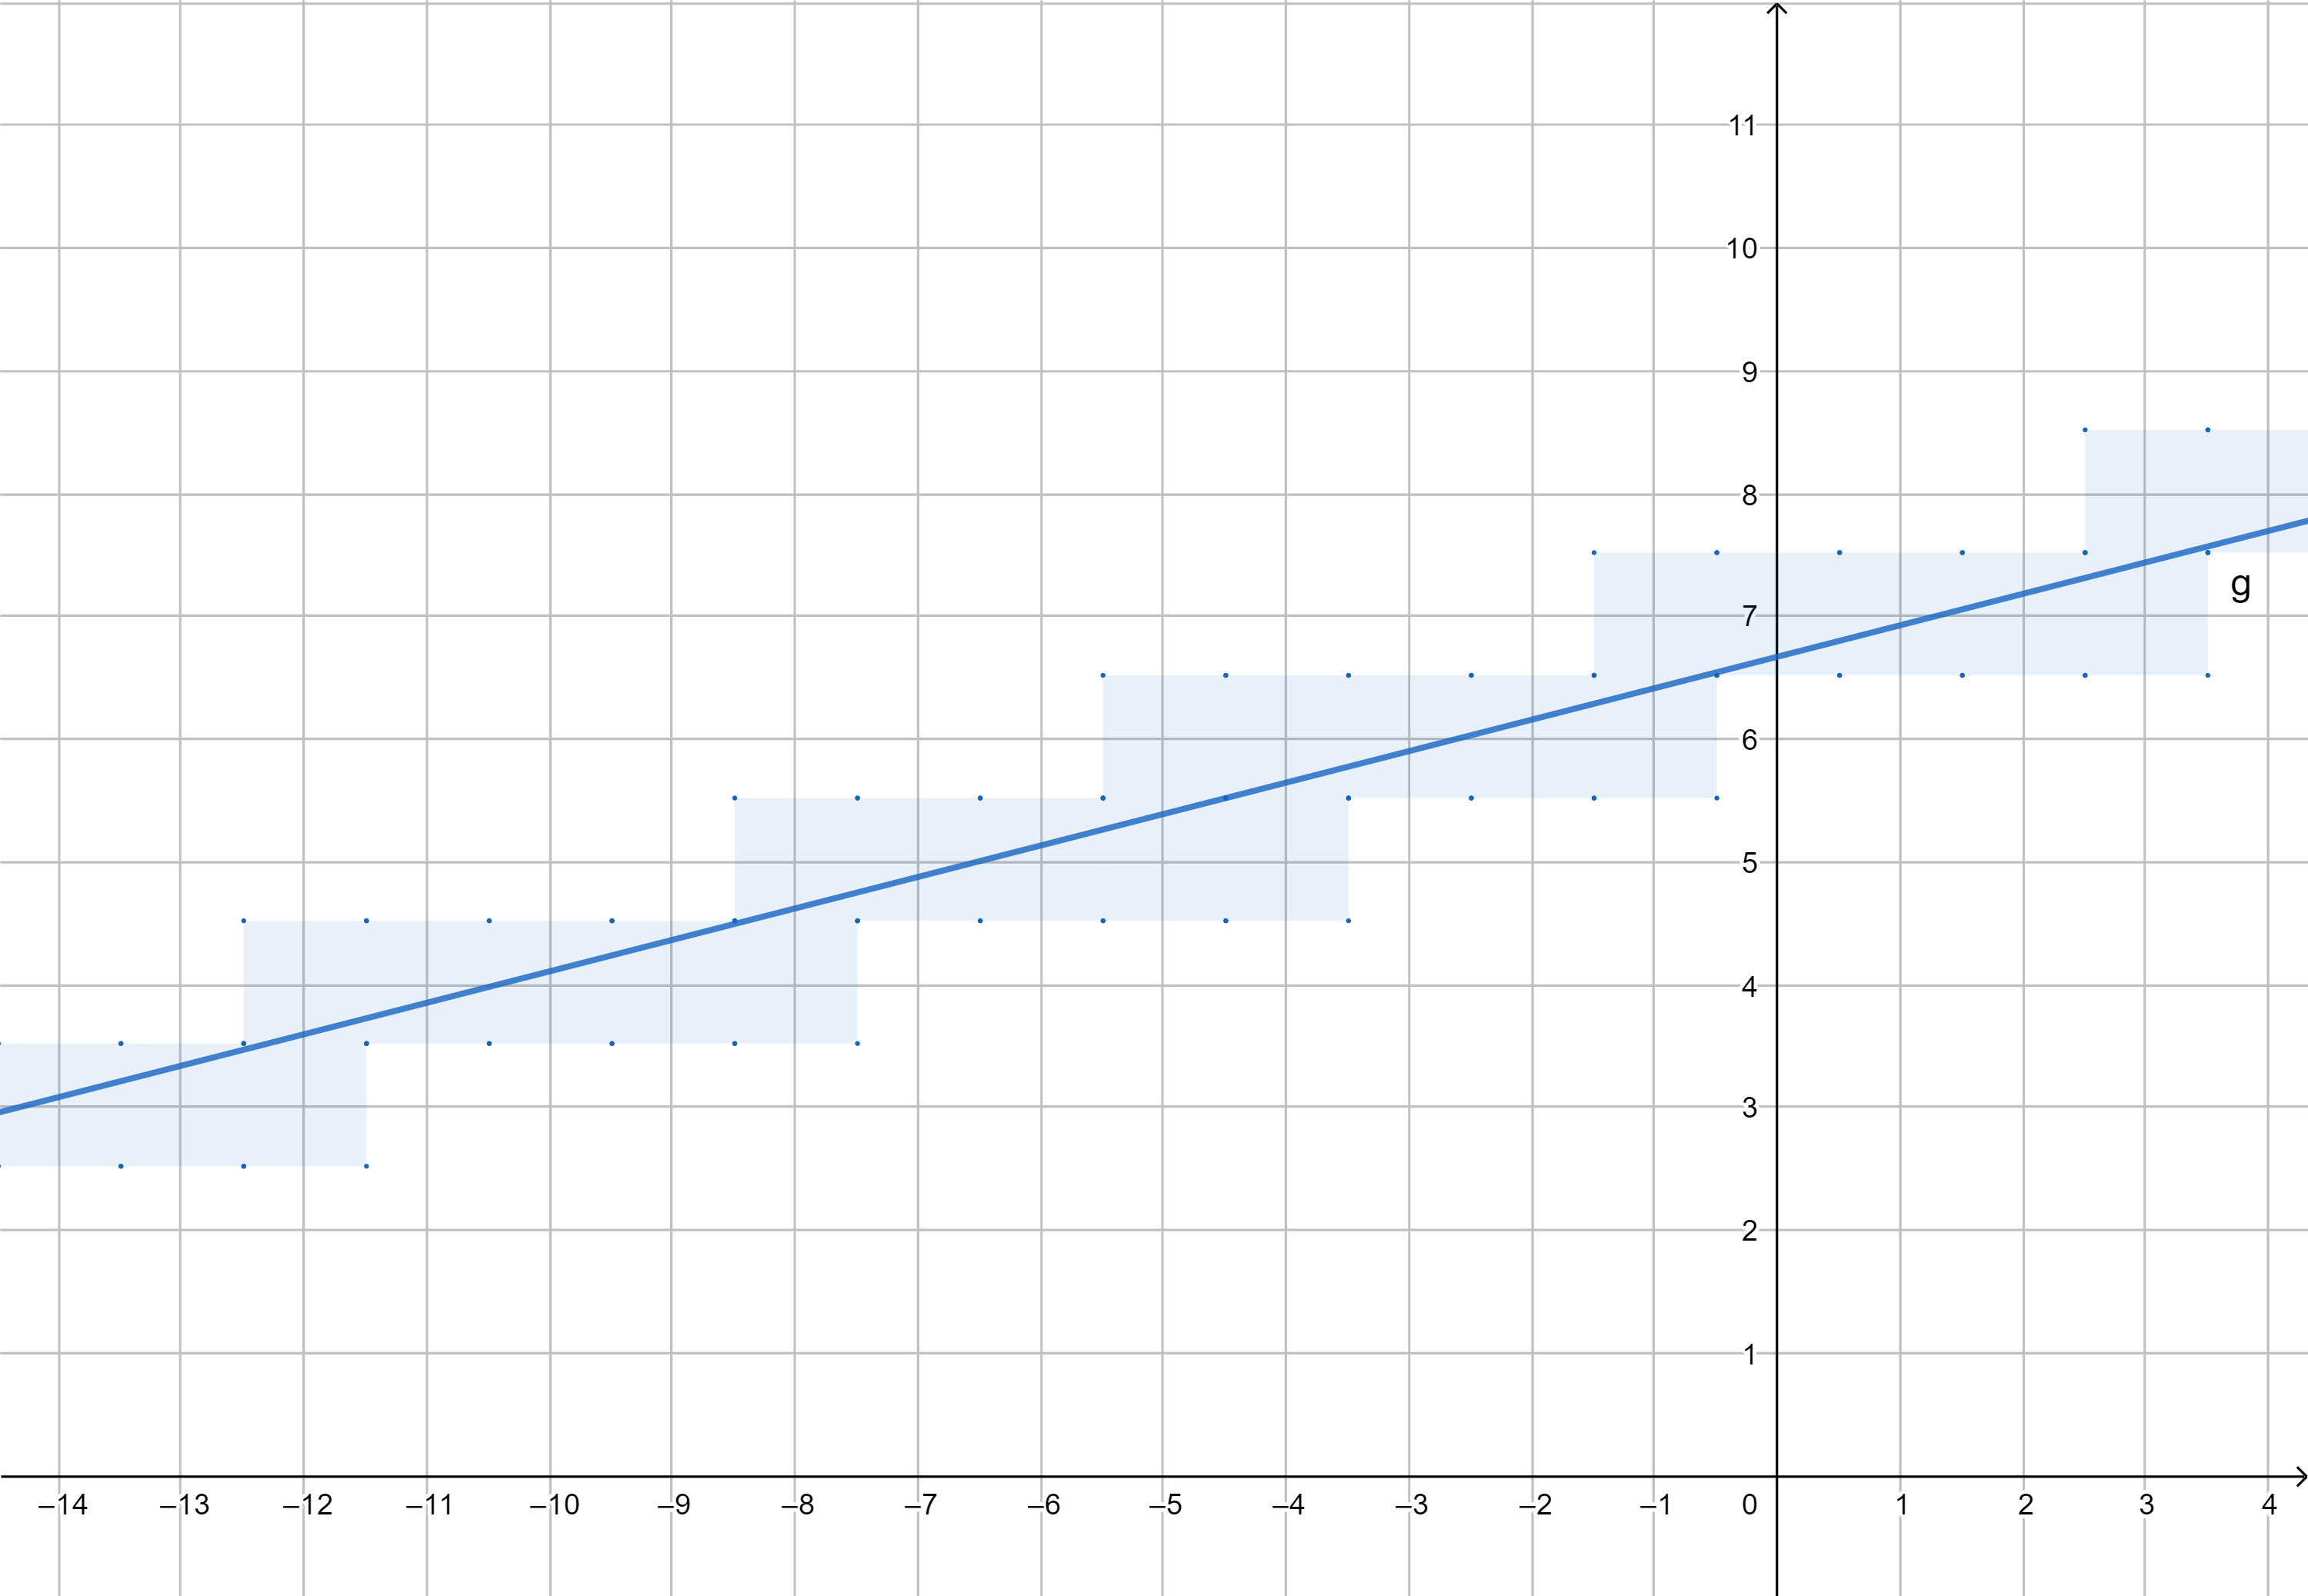
\includegraphics[height=10cm]{line-hit-squares.png}
	\caption{$g$ hits squares around points} \label{linesquares}
	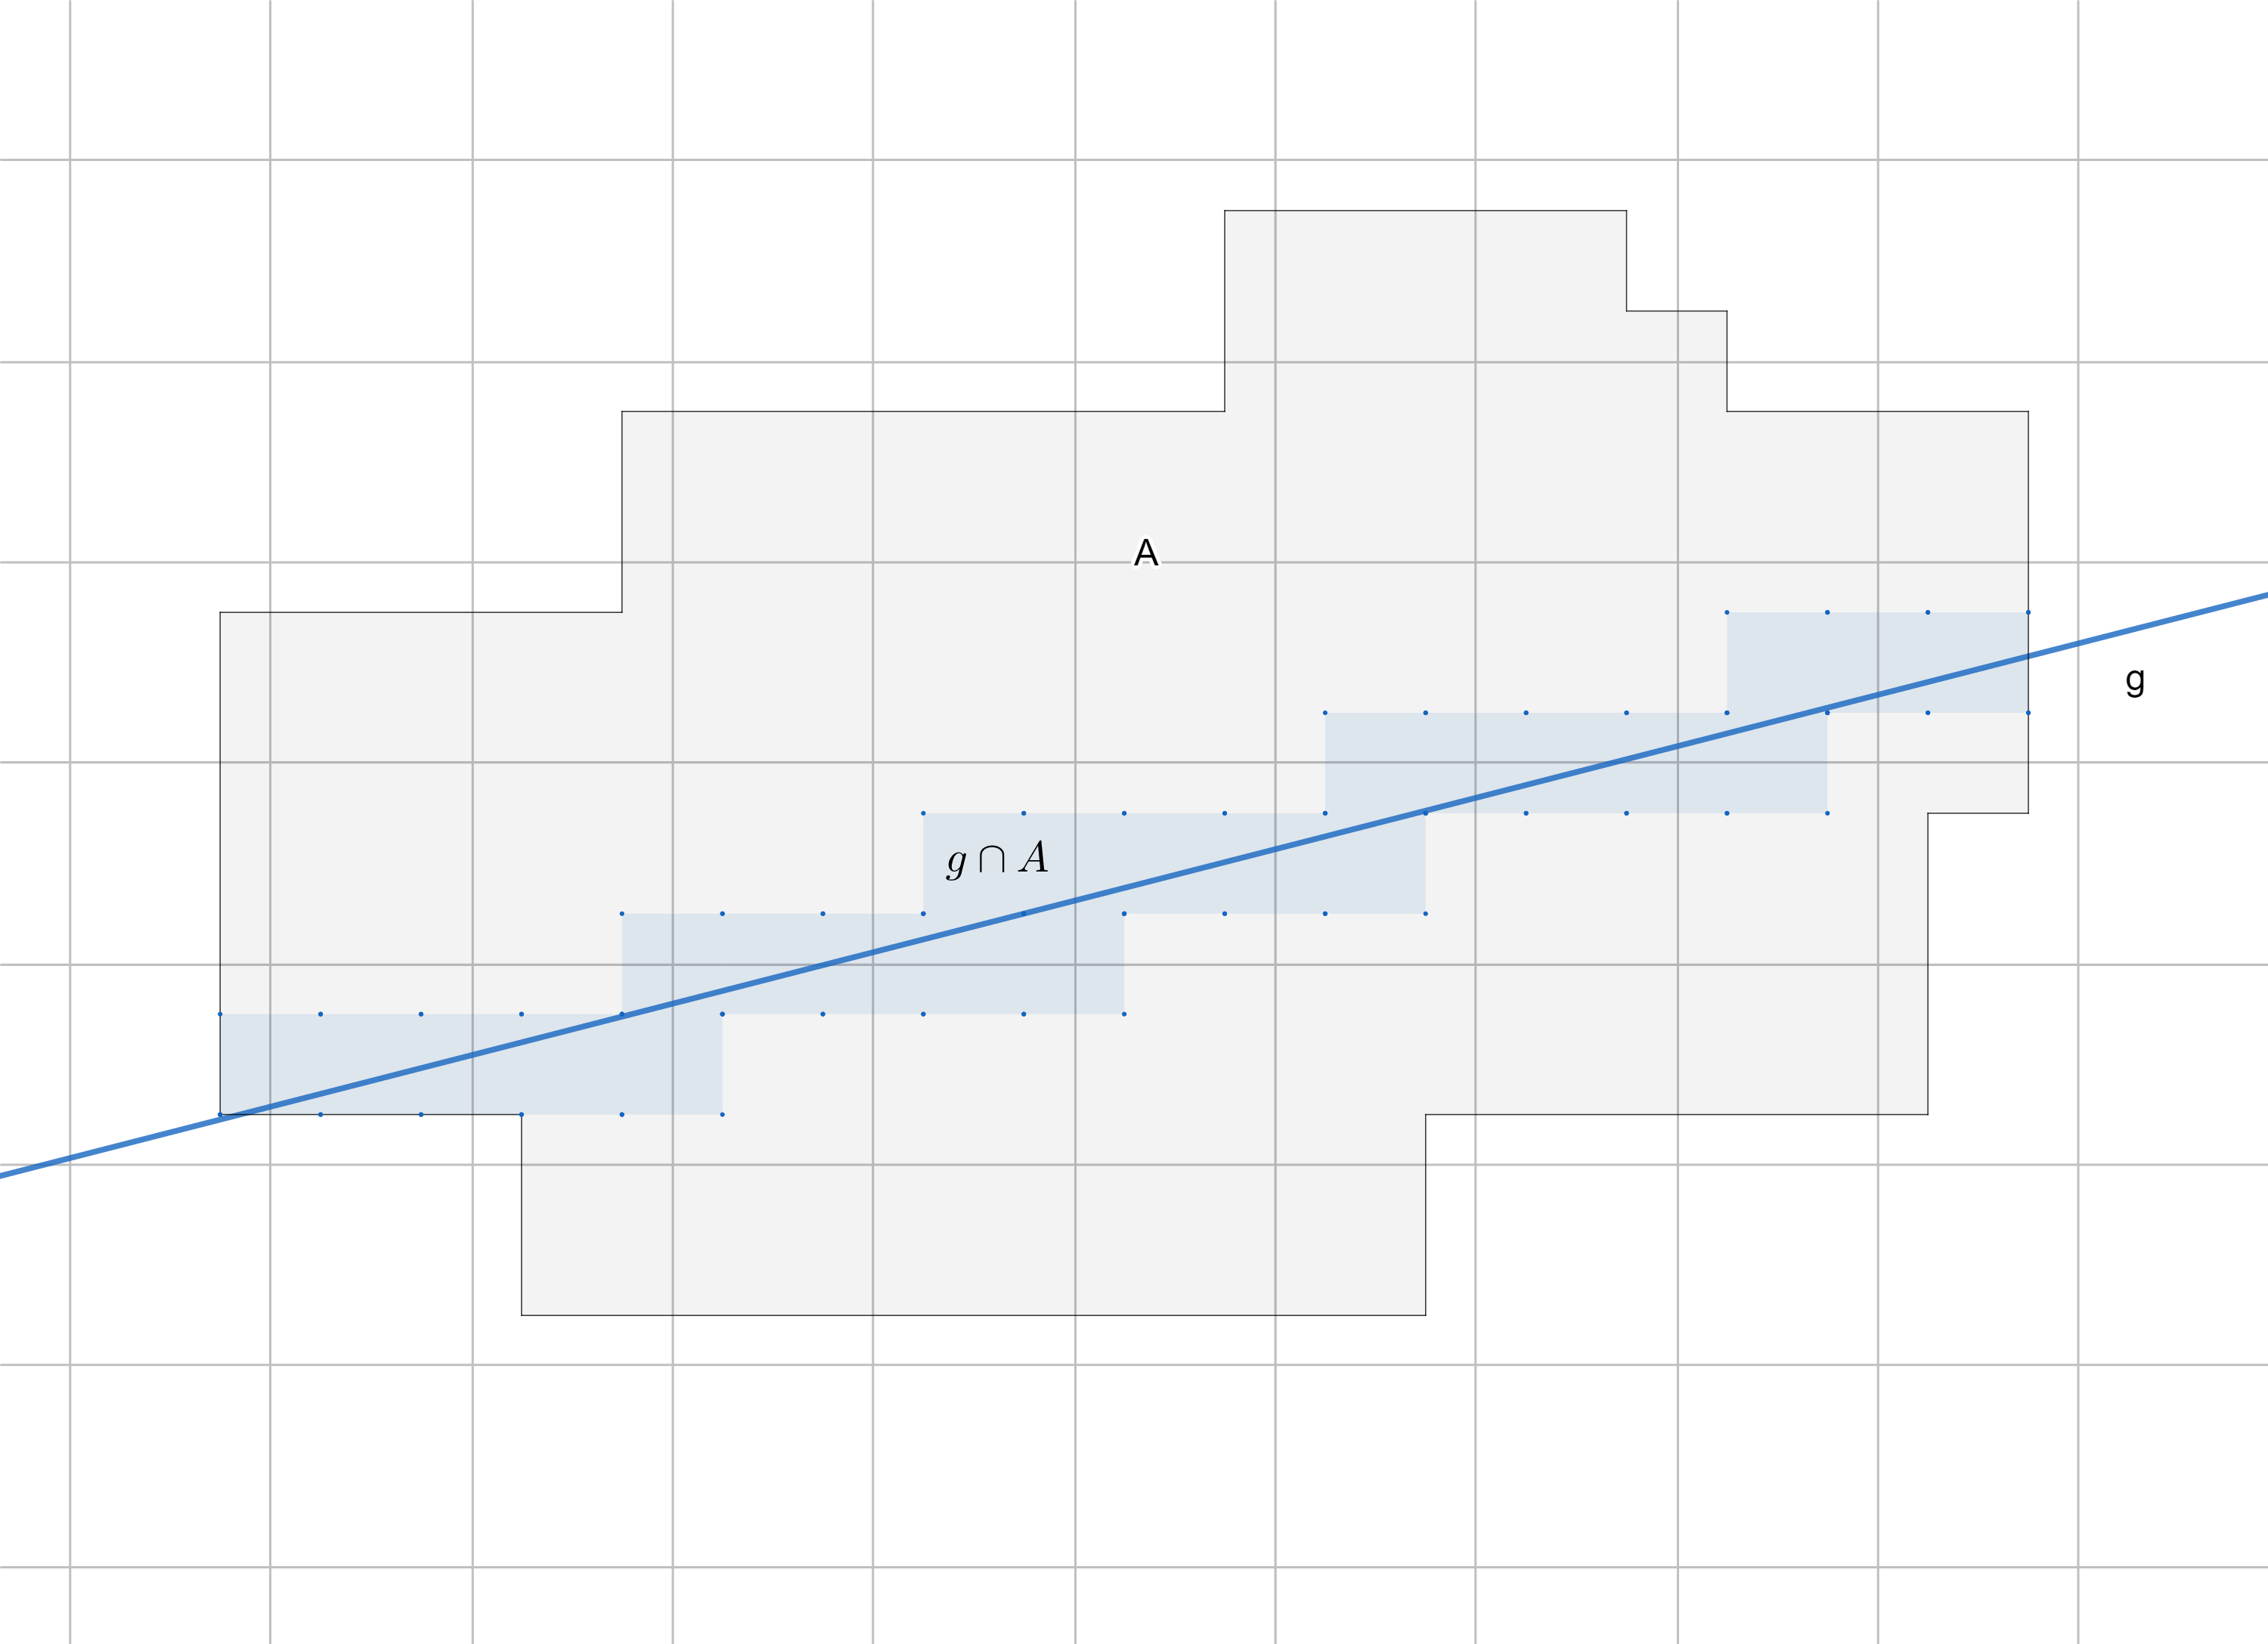
\includegraphics[height=10cm]{line-hit-A.png}
	\caption{$g$ hits squares in $A$} \label{linesquaresA}
\end{figure}

\begin{definition}
	Let $g=g_{\alpha,p}\in \G$ and $A\in \mathcal{P}_f$. We define 
	
	\begin{align*}
		g\cap A := \{ p\in A\ |\ g \text{ hits } p\}
	\end{align*}
	
	which is the subset of all points in $A$ which are hit by $g$ (see $\autoref{linesquaresA}$). For the following we suppose $g\cap A \neq \emptyset$. We will define a total ordered relation $\triangleleft$ on $g\cap A$ which shall be defined equivalently for all $g\in \G$ and $A\in\mathcal{P}_f$ with $g\cap A \neq\emptyset$. We choose two points $x,y\in g\cap A$ and split the definition of the relation $\triangleleft$ into four cases, depending on whether the line $g$ goes from left-bottom to right-top, left-top to right-bottom, parallel to the $x$-axis and parallel to the $y$-axis. Denote the real part of $x$ with $Re(x)$ and the imaginary one with $Im(x)$. \\
	\\
	$\mathit{Case}\ 1:\quad g\ \text{ is parallel to the x-axis}\quad (\Leftrightarrow\quad \alpha = \frac{\pi}{2})$
	\begin{align*}
	x \triangleleft y \quad :\Leftrightarrow \quad Re(x) < Re(y)
	\end{align*}\\
	$\mathit{Case}\ 2:\quad g\ \text{ is parallel to the y-axis}\quad (\Leftrightarrow\quad \alpha = 0)$
	\begin{align*}
	x \triangleleft y \quad :\Leftrightarrow \quad Im(x) < Im(y)
	\end{align*}\\
	$\mathit{Case}\ 3:\quad g\ \text{ is going from left-bottom to right-top}\quad (\Leftrightarrow\quad \alpha\in (\frac{\pi}{2},\pi))$
	\begin{align*}
	x \triangleleft y \quad :\Leftrightarrow \quad
		\begin{cases}
			Re(x) < Re(y), & \text{ if } Re(x) \neq Re(y), \\
			Im(x) < Im(y), & \text{ if } Re(x) = Re(y).
		\end{cases}
	\end{align*}\\
	$\mathit{Case}\ 4:\quad g\ \text{ is going from left-top to right-bottom}\quad (\Leftrightarrow\quad \alpha\in (0,\frac{\pi}{2}))$
	\begin{align*}
	x \triangleleft y \quad :\Leftrightarrow \quad
	\begin{cases}
	Re(x) < Re(y), & \text{ if } Re(x) \neq Re(y), \\
	Im(x) > Im(y), & \text{ if } Re(x) = Re(y).
	\end{cases}
	\end{align*}\\
	It is easy to see that this relation on $g\cap A$ is well-defined. In the following we will prove that this relation is strictly and totally ordered. 
\end{definition}

\begin{lemma}
For a line $g=g_{\alpha,p}\in\G$ and $A\in \mathcal{P}_f$ with $g\cap A\neq \emptyset$ the relation $\triangleleft$ on $g\cap A$ is totally ordered. 
	\begin{proof}
		We will only proove the case where $g$ is going from left-bottom to right-top, which is $\mathit{Case}\ 3$ of the definition. In this case we have $\alpha\in (\frac{\pi}{2},\pi)$. Note, that the proof for $\mathit{Case\ }4$ will work very similair and in the case of $g$ being parallel to one of the axes ($\mathit{Case\ }1$ or $2$), all properties for a totally ordered relation follow directly from the totally ordered relation $<$ on $\mathbb{R}$. So let $\alpha\in (\frac{\pi}{2},\pi)$. \\
		\\
		$\mathit{Antisymmetry:}$ For antisymmetry let $x \triangleleft y$ and $y \triangleleft x$. Suppose $Re(x)\neq Re(y)$, then $Re(x) < Re(y)$ and $Re(y) < Re(x)$, a contradiction because of the total order $<$ in $\mathbb{R}$. So $Re(x) = Re(y)$. But then we have $Im(x) < Im(y)$ and $Im(y) < Im(x)$ and therefore also $Im(x) = Im(y)$, hence $x=y$. \\
		\\
		$\mathit{Transitivity:}$ For transitivity let $x \triangleleft y$ and $y \triangleleft z$. We find four cases. In case $Re(x) \neq Re(y)$ and $Re(y) \neq Re(z)$ we get $Re(x) < Re(z)$ by transitivity of $<$, hence $x \triangleleft z$. In case $Re(x)\neq Re(y)$ and $Re(y) = Re(z)$ we get $Re(x) < Re(y) = Re(z)$, therefore $x \triangleleft z$. In case $Re(x) = Re(y)$ and $Re(y) \neq Re(z)$ we get $Re(x) = Re(y) < Re(z)$, similair as the last case. In the last case $Re(x) = Re(y) = Re(z)$ we get $Im(x) < Im(y)$ and $Im(y) < Im(z)$ and again by transitivity of $<$ we get $Im(x) < Im(z)$, hence $x \triangleleft z$ again. \\
		\\
		$\mathit{Connexity:}$ Connexity is given since for any two points $x,y\in g\cap A$ we have either $Re(x) \neq Re(y)$ or $Re(x) = Re(y)$ and therefore either $x\triangleleft y$ or $y\triangleleft x$.
	 
	\end{proof}
\end{lemma}

\begin{remark}
	The relation $\triangleleft$ on $g\cap A$ basically orders the hitting points of $g$ with $A$ from left to right (or bottom to top in case of a line parallel to the $y$-axis). This order allows us to identify the outermost hitting points which are the minimum and maximum of $g\cap A$ with respect to $\triangleleft$. To clarify, we define $\min (g\cap A) := x_0$ if and only if $x_0 \triangleleft x$ for all $x\in g\cap A,x\neq x_0$, analogously $\max(g\cap A)$. This means when moving on $g$ facing $A$ coming from infinity this order allows to know where in $A$ the line $g$ hits first when "entering" $A$ and where it hits last when "leaving" $A$. 
\end{remark}

Recall that for a bounded subset $A\subset \C$ the convex hull $conv(A)$ of $A$ is defined to be the smallest convex set containing $A$, formally 
\begin{flalign*}
	conv(A) := \bigcap_{A\subset K\in \K^2} K. 
\end{flalign*}
Note that $conv(A)\in \K^2$ for all bounded subsets $A\subset \C$. For a set $A\in \mathcal{P}_f$ we define 
\begin{flalign*}
	conv(A):=conv(\bigcup_{p\in A} sq(p))
\end{flalign*}
and since $\bigcup_{p\in A} sq(p)$ is a bounded set we have $conv(A)\in \K^2$. 

\begin{definition} $\mathit{(Random\ Line\ Hitting\ Distribution)}$ Let $A\in \mathcal{P}_f$ and $K := conv(A)\in \K^2$. For $x\in\Z^2$ and $g\in \G$ define
	\begin{flalign*}
		\tilde \mu_A(x,g) := (\frac{1}{2}\1\{|g\cap A| \geq 2\} + \1\{|g\cap A| = 1\}) \ \1\{x\in \{\min(g\cap A),\max(g\cap A)\}\}
	\end{flalign*}
	and
	\begin{flalign}
		\mu_A(x) := \frac{1}{\PP^K_\mu([A])} \int_\G \ \tilde \mu_A(x,g) \ \PP^K_\mu(dg).
	\end{flalign}
	We quickly show that $\mu_A\in \mathcal{D}_A$. For all $x\in \Z^2\setminus A$ and $g\in \G$ we have $\tilde \mu_A(x,g) = 0$ and therefore $\mu_A(x) = 0$. Furthermore for all $g\in \G$ we have
	\begin{flalign*}
		\sum_{x\in A} \tilde \mu_A(x,g) = \begin{cases}
			\frac{1}{2}2, \quad &|g\cap A| \geq 2, \\
			1, \quad &|g\cap A| = 1, \\
			0, \quad &|g\cap A| = 0.
		\end{cases} \quad= \1\{g\cap A\neq \emptyset\}
	\end{flalign*} 
	and therefore 
	\begin{flalign*}
		\sum_{x\in A} \mu_A(x) = \frac{1}{\PP^K_\mu([A])}\ \int_\G \1\{g\cap A\neq \emptyset\}\ \PP^K_\mu(dg) = \frac{\PP^K_\mu([A])}{\PP^K_\mu([A])} = 1. 
	\end{flalign*}
	Hence, the family of distributions $(\mu_A)_{A\in \mathcal{P}_f}$ defines an incremental aggregate. 
\end{definition}

\begin{definition} $(\mathit{Line\ Hitting\ Aggregate)}$ An Incremental Aggregate with the Random Line Hitting Distribution we call $\mathit{Line\ Hitting\ Aggregate}$, short $\mathit{LHA}$. 
\end{definition}

\newpage
\section{Python Simulation}
Part of the work in this paper is the attempt to build simulations for both incremental aggregates $\mathit{External\ DLA}$ and $\mathit{LHI}$ which were presented in the previous sections. For calculating the simulations we use $\mathit{Python}$ and for rendering pictures we use the package $\mathit{Pygame}$. Each vertex in $\Z^2$ is naturally mapped to its coordinate and is represented in this way in python code. In graphics each coordinate basically can be represented by squares in $\C$ as presented in Definition $\ref{squares}$, and each square will be represented by exactly one pixel, so every picture about incremental aggregates you'll see in the following consists of pixels each representing exactly one vertex in $\Z^2$ in the most natural way. Our aim will be to simulate the aggregates as close as possible to their mathematical definitions. This is much easier for LHI, and less obvious for External DLA. We start of with External DLA in the following.

\subsection{External DLA Simulation}

By identifying each vertex in $\Z^2$ with its square in $\C$ and a pixel when rendering, the representation of the space we are moving is exact. For any simulation of randomness we use the package $\mathit{random}$. Respecting the error behaviour of this package, random walks on $\Z^2$ can be simulated directly and therefore very exact. For External DLA we let a particle move randomly on the grid and wait for it to hit the actual cluster. The problem which will have to be solved is where to start the moving particle and how to handle a particle when it is moving away from the actual cluster, therefore creating a too long waiting time for it coming back to the cluster. In the definition of External DLA new particles start the random walk from infinity. Obviously this is not possible in simulation so this has to be solved differently. 



\subsection{LHI Simulation}



\newpage
\section{Questions}

\newpage

\begin{thebibliography}{biblio}
\thispagestyle{empty}

\bibitem{Henze Skript}
N. Henze.
\emph{Maß und Wahrscheinlichkeitstheorie (Stochastik II)}.
Karlsruher Institut für Technologie, Karlsruhe, 2010

\bibitem{stoch1}
Daniel Hug, Günter Last, Steffen Winter.
\emph{Stochastic Geometry, 	Lecture Notes (summer term 2020)}.
Institute of Technology, Karlsruhe, 2020

\bibitem{sackmann}
Franz Sackmann. 
\emph{Zufällige Geraden, Staatsexamensarbeit}.
University Karlsruhe (TH), Karlsruhe, 2007



\end{thebibliography}

\newpage
  
\thispagestyle{empty}

\vspace*{8cm}


\section*{Erklärung}

Hiermit versichere ich, dass ich diese Arbeit selbständig verfasst und keine anderen als die angegebenen Quellen und Hilfsmittel benutzt, die wörtlich oder inhaltlich übernommenen Stellen als solche kenntlich gemacht und die Satzung des Karlsruher Instituts für Technologie zur Sicherung guter wissenschaftlicher Praxis in der jeweils gültigen Fassung beachtet habe. \\[2ex] 

\noindent
Karlsruhe, den 10. März 2020\\[5ex] 

\end{document}

